
\chapter{Runtime Overheads Migration}
\label{chapter.taskgenx}
As chip multi-processors (CMPs) are becoming more and more complex, software solutions such as parallel programming models are attracting a lot of attention.
Task-based parallel programming models offer an appealing approach to utilize complex CMPs.
However, the increasing number of cores on modern CMPs is pushing research towards the use of fine grained parallelism.
Task-based programming models need to be able to handle such workloads and offer performance and scalability.
Using specialized hardware for boosting performance of task-based programming models is a common practice in the research community.

This chapter makes the observation that task creation becomes a bottleneck when we execute fine grained parallel applications with task-based programming models.
As the number of cores increases the time spent generating the tasks of the application is becoming more critical to the entire execution.
To overcome this issue, we propose {\proposal}.
{\proposal} offers a solution for minimizing task creation overheads and relies both on the runtime system and a dedicated hardware.
%We propose \proposal, a task-based programming model that offers a minimalistic approach to runtime overheads acceleration.
On the runtime system side, {\proposal} decouples the task creation from the other runtime activities.
It then transfers this part of the runtime to a specialized hardware.
We draw the requirements for this hardware in order to boost execution of highly parallel applications.
From our evaluation using 11 parallel workloads on both symmetric and asymmetric systems, we obtain performance improvements up to 15$\times$, averaging to 3.1$\times$ over the baseline.
\newpage

%%%%%%%%%%%%%%%%%%%
%%%%%%%%%%%%%%%%%%%
\section{Introduction}
\label{sec:intro}

%%%%%%%%%%%%%%%%%%%%%%%%%%%
%%%%%%%%%%%%%%%%%%%%%%%%%%%
Since the end of Dennard scaling~\cite{Dennard74} and the subsequent stagnation of CPU clock frequencies, computer architects and programmers rely on multi-core designs to achieve the desired performance levels.
While multi-core architectures constitute a solution to the CPU clock stagnation problem, they bring important challenges both from the hardware and software perspectives.
On the hardware side, multi-core architectures require sophisticated mechanisms in terms of coherence protocols, consistency models or deep memory hierarchies. 
Such requirements complicate the hardware design process.
On the software side, multi-core designs significantly complicate the programming burden compared to their single-core predecessors.
The different CPUs are exposed to the programmer, who has to make sure to use all of them efficiently, as well as using the memory hierarchy properly by exploiting both temporal and spatial locality.
This increasing programming complexity, also known as the Programmability Wall~\cite{Chapman2007}, has motivated the advent of sophisticated programming paradigms and runtime system software to support them.

Task-based parallelism~\cite{Blumofe:PPoPP1995, Reinders2007, Bauer2012, OmpSs} has been proposed as a solution to the Programmability Wall and, indeed, the most relevant shared memory programming standards, like OpenMP, support tasking constructs~\cite{OpenMP4.0:Manual2015}.
The task based model requires the programmer to split the code into several sequential pieces, called tasks, as well as explicitly specifying their input and output dependencies. 
%It also requires these pieces of code to be annotated in terms of input or output data dependencies.
The task-based execution model (or runtime system) consists of a master thread and several worker threads. The master thread goes over the code of the application and creates tasks once it encounters source code annotations identifying them. 
The runtime system manages the pool of all created tasks and schedules them across the threads once their input dependencies are satisfied.
To carry out the task management process, the parallel runtime system creates and maintains a Task Dependency Graph (TDG).
In this graph nodes represent tasks and edges are dependencies between them.
Once a new task is created, a new node is added to the TDG. 
The connectivity of this new node is defined by the data dependencies of the task it represents, which are explicitly specified in the application's source code.
When the execution of a task finalizes, its corresponding node is removed from the TDG, as well as its data dependencies.

This task-based runtime system constitutes of a software layer that enables parallel programmers to decouple the parallel code from the underlying parallel architecture where it is supposed to run on.
As long as the application can be decomposed into tasks, the task-based execution model is able to properly manage it across homogeneous many-core architectures or heterogeneous designs with different core types. 
A common practice in the high performance domain is to map a single thread per core, which enables the tasks running on that thread to fully use the core capacity. 
Finally, another important asset of task-based parallelism is the possibility of automatically managing executions on accelerators with different address spaces. 
Since the input and output dependencies of tasks are specified, the runtime system can automatically offload a task and its dependencies to an accelerator device (e.g., GPU) without the need for specific programmer intervention~\cite{Bueno:IPDPS2012}.
Additional optimizations in terms of software pre-fetching~\cite{Papaefstathiou2013} or more efficient coherence protocols~\cite{Manivannan2014} can also be enabled by the task-based paradigm.

Despite their advantages, task-based programming models also induce computational costs.
For example, the process of task creation requires the traversal of several indexed tables to update the status of the parallel run by adding the new dependencies the recently created tasks bring, which produces a certain overhead.
Such overhead constitutes a significant burden, especially on architectures with several 10's or 100's of cores where tasks need to be created at a very fast rate to feed all of them.
This paper proposes the Task Generation Express ({\proposal}) approach. 
Our proposal suggests that the software and hardware are designed to eliminate the most important bottlenecks of task-based parallelism without hurting their multiple advantages. 
This paper focuses on the software part of this proposal and draws the requirements of the hardware design to achieve significant results.
%This paper proposes the Task Generation Express ({\proposal}) approach, a combined hardware-software solution to eliminate the most important bottlenecks of task-based parallelism without hurting their multiple advantages.
In particular, this paper makes the following contributions beyond the state-of-the-art:

\begin{itemize}

\item A new parallel task-based runtime system that decouples the most costly routines from the other runtime activities and thus enables them to be off-loaded to specific-purpose helper cores.

\item A detailed study of the requirements of a specific-purpose helper core able to accelerate the most time consuming runtime system activities. 
%To accelerate the time consuming runtime parts,
%\item A specific-purpose helper core able to accelerate the most time consuming runtime system activities. This hardware is also able to run user-level tasks, although it does so in a very slow way compared to a general purpose core.

\item A complete evaluation via trace-driven simulation considering 11 parallel OpenMP codes and $25$ different system configurations, including homogeneous and heterogeneous systems. %and large core counts up to $XXX$ cores. 
Our evaluation demonstrates how {\proposal} achieves average speedups of $3.1\times$ when compared against currently use state-of-the-art approaches.

\end{itemize} 

The rest of this chapter is organized as follows: 
Section~\ref{sec.taskgenx.background} describes the task-based execution model and its main bottlenecks.
Section~\ref{sec.taskgenx.ram} describes the new task-based runtime system this paper proposes as well as the specialized hardware that accelerates the most time-consuming runtime routines.
Section~\ref{sec.taskgenx.evaluation} describes the evaluation of {\proposal} via trace-driven simulation and Section~\ref{sec.taskgenx.conclusions} concludes this work.




%%%%%%%%%%%%%%%%%%%
%%%%%%%%%%%%%%%%%%%
\section{Background and Motivation}
\label{sec.taskgenx.background}
\lstset{basicstyle=\small\ttfamily,
        emphstyle=\bfseries,
        columns=fixed,
        numbers=left,xleftmargin=2em,frame=single,framexleftmargin=1.5em,
        moredelim=*[l][\textit]{//},
        moredelim=*[l][\bfseries]{\#},
        literate={...}{\dots}3
} 
\subsection{Task-based Programming Models}
\label{sec.background}
\begin{lstlisting}[float, emph={void,if,return,Dependency,DepList,Data,not,true,and,break}, captionpos=b, caption={Compiler generated pseudo-code equivalence for task annotation.},label=task_clause, emph={[2]mat}, emphstyle={[2]}, aboveskip={0\baselineskip}, frame=tb, belowskip={0\baselineskip}]
     ...
  //task_clause
  memalloc(&task, args, size);
  createTask(deps, task, parent, taskData);
     ...
\end{lstlisting}
\begin{lstlisting}[float, emph={is, void,if,return,Dependency,DepList,Data,Task,not,true,and,break}, captionpos=b, caption={Pseudo-code for task creation.},label=taskCreation, emph={[2]mat}, emphstyle={[2]}, aboveskip={0\baselineskip}, frame=tb, belowskip={0\baselineskip}]
void createTask(DepList dList, Task t,  
                Task parent, Data args) {
  initAndSetupTask(task1, parent, args);
  insertToTDG(dList, task1);
}
\end{lstlisting}

Task-based parallel programming models ~\cite{Blumofe:PPoPP1995, Reinders2007, Bauer2012, OmpSs},  are widely used to facilitate the programming of parallel codes for multi-core systems.
These programming models offer annotations that the programmer can add to the application's sequential code.
One type of these annotations is the task annotations with dependency tracking which OpenMP~\cite{OpenMP} supports since its 4.0 release~\cite{OpenMP4.0:Manual2015}. 
By adding these annotations, the programmer decomposes the application into \textit{tasks} and specifies the input and output data dependencies between them. 
A compiler is responsible to translate the annotations into code by adding calls to the programming model's runtime system. 
The runtime system consists of software threads and is responsible for the efficient execution of the tasks with respect to the data dependencies as well as the availability of resources.

When the compiler encounters a task annotation in the code, it transforms it to the pseudo-code shown in Listing~\ref{task_clause}.
\texttt{Memalloc} is performing the memory allocation for the task and its arguments.
Next is a runtime call, which is the \texttt{createTask}, responsible for the linking of the task with the runtime system.
At this point a task is considered \textit{created} and below are the three possible states of a task inside the runtime system:
\begin{itemize}
\item \textit{Created:} A task is initialized with the appropriate data and function pointers and it is inserted in the Task Dependency Graph (TDG). The insertion of a task in the TDG implies that the data dependencies of the tasks have been identified and the appropriate data structures have been created and initialized. 
%At this point a task is considered as \textit{created} but not \textit{ready}.
%\item \textit{TDG Submission:} After the allocation, a task is being inserted in the Task Dependency Graph (TDG). The insertion of a task in the TDG implies that the data dependencies of the tasks have been identified and the appropriate data structures have been created and properly initialized. At this point a task is considered as \textit{created} but not \textit{ready}.
\item \textit{Ready:} When all the data dependencies of a created task have been satisfied, the task is ready and it is inserted in the \textit{ready queue} where it waits for execution. 
\item \textit{Finished:} When a task has finished execution and has not been deleted yet.
\end{itemize}

The runtime system creates and manages the software threads for the execution of the tasks. 
Typically one software thread is being bound to each core. 
One of the threads is the \textit{master thread}, and the rest are the \textit{worker threads}. 
The master thread starts executing the code of Listing~\ref{task_clause} sequentially. 
The allocation of the task takes place first.
What follows is the task creation, that includes the analysis of the dependencies of the created task and the connection to the rest of the existing dependencies.
Then, if there are no task dependencies, which means that the task is \textit{ready}, the task is also inserted in the ready queue and waits for execution.
\begin{lstlisting}[float, emph={is, void,if,return,Dependency,DepList,Data,Task,not,for,true,and,break}, captionpos=b, caption={Pseudo-code for TDG insertion},label=insertTDG, emph={[2]mat}, emphstyle={[2]}, aboveskip={0\baselineskip}, frame=tb, belowskip={0\baselineskip}]
void insertToTDG(DepList dList, Task t) {
  if( dList is empty ) {
    readyQ->push(t);
    return;
  }
  Dependency entry;
  for( d in dList ) {
    entry = depMap[d.address()];
    if(entry==NULL) depMap.add(entry, t);
    if(d.accessType() == "write")
      entry.addLastWriter(t);
    if(d.accessType() == "read") {
        entry.addReader(t);
        entry.lastWriter()->addSuccessor(t);
    }
  }
}
\end{lstlisting}
Listing~\ref{taskCreation} shows the pseudo-code for the task creation step within the runtime.
The \texttt{createTask} function is first initializing the task by copying the corresponding data to the allocated memory as well as connecting the task to its parent task (\texttt{initAndSetupTask}).
After this step, the task is ready to be inserted in the TDG. 
The TDG is a distributed and dynamic graph structure that the runtime uses to keep the information about the current tasks of the application. 
The insertion of a task in the TDG is done by the \texttt{insertToTDG} function.
This function takes as arguments a list with all the memory addresses that are to be written or read by the task (\texttt{dList}), and the task itself.
Listing~\ref{insertTDG} shows the pseudo-code for the TDG insertion. 
If for a task the \texttt{dList} is empty (line 2), this means that there are no memory addresses that need to be tracked during the execution; thus, the task is marked as \textit{ready} by pushing it to the \textit{ready queue} (line 3).
Each entry of \texttt{dList} contains the actual memory address as well as the access type (read, write or read-write).
The runtime keeps a distributed unified dependency tracking structure, the \texttt{depMap} where it stores all the tracked memory addresses together with their writer and reader tasks.
For each item in the \texttt{dList} the runtime checks if there is an existing representation inside the \texttt{depMap} (line 8).
If the memory address of an entry of the \texttt{dList} is not represented in the \texttt{depMap}, it is being added as shown in line 9.
If the address of a \texttt{dList} item exists in the \texttt{depMap}, this means that a prior task has already referred to this memory location, exhibiting a data dependency.
According to the access type of \texttt{d}, the readers and the writers of the specific address are updated in the \texttt{depMap} (lines 10-15).

To reduce the lookup into the \texttt{depMap} calls, every time the contents of a memory address are modified, the tasks keep track of their \textit{successors} as well as the number of \textit{predecessors}.
The \textit{successors} of a task are all the tasks with inputs depending on the output of the current task.
The \textit{predecessors} of a task are the tasks whose output is used as input for the current task.
When a \texttt{read} access is identified, the task that is being created is added to the list of successors of the last writer task, as shown on line 20 of Listing~\ref{taskCreation}.

\begin{lstlisting}[float, emph={void,if,return,Task,for,not,true,and,break}, captionpos=b, caption={Pseudo-code for task$\_$finish runtime activity.},label=taskFinish, emph={[2]mat}, emphstyle={[5]}, aboveskip={0\baselineskip}, frame=tb, belowskip={0\baselineskip}]
void task_finish(Task *t) {
  depMap.removeReaderWriter(t);
  if(t->successors.empty()) delete t;
  else {
    for( succ in t->successors ) {
        succ.decreasePredecessors();
        if(succ.numPredecessors == 0) 
            readyQ->push(succ);
    }
  }
}
\end{lstlisting}

As tasks are executed, the dependencies between them and their successors are satisfied. 
So the successor tasks that are waiting for input, eventually become \textit{ready} and are inserted to the ready queue.
When a task goes to the \textit{finished} state, the runtime has to perform some actions in order to prepare the successor tasks for execution.
These actions are described in Listing~\ref{taskFinish}.
The runtime first updates the \texttt{depMap} to remove the possible references of the task as reader or writer (line 2).
Then, if the task does not have any successors, it can safely be deleted (line 3).
If the task has successors, the runtime traverses the successor list and for each successor task it decreases its predecessor counter (lines 5-6).
If for a successor task its predecessor counter reaches zero, then this task becomes \textit{ready} and it is inserted in the \textit{ready queue} (lines 7-8).

The runtime activity takes place at the task state changes. 
One state change corresponds to the task creation, so a task from being just allocated it becomes \textit{created}. 
At this point the runtime prepares all the appropriate task and dependency tracking data structures as well as inserts the task into the TDG.
The second change occurs when a task from being \textit{created} it becomes \textit{ready};
this implies that the input dependencies of this task are satisfied so the runtime schedules and inserts the task into the ready queue.
The third change occurs when a running task finishes execution. 
In this case, following our task states, the task from being \textit{ready} it becomes \textit{finished}; this is followed by the runtime updating the dependency tracking data structures and scheduling possible successor tasks that become ready. 
For the rest of the paper we will refer to the first state change runtime activity as the task creation overheads (\textit{Create}).
For the runtime activity that takes place for the following two state changes (and includes scheduling and dependence analysis) we will use the term runtime overheads (\textit{Runtime}).



%\begin{lstlisting}[float, emph={void,if,return,not,true,and,break}, captionpos=b, caption={Pseudo-code for task creation.},label=taskCreation, emph={[2]mat}, emphstyle={[2]}, aboveskip={0\baselineskip}, frame=tb, belowskip={0\baselineskip}]
%
%void createTask(Deplist dList, Task task1, 
%            Task parent, Data taskData) {
%  initAndSetupTask(task1, parent, taskData);
%  insertToTDG(dList, task1);
%}
%
%Dependency depMap[];
%
%void insertToTDG(DepList dList, Task task1) {
% if( dList.empty() ) {
%   rQueue_submission(task1);
%   return;
% }
% Dependency entry;
% for( d in dList ) {
%   entry = depMap.lookupAddress(d.address());
%   if(entry == NULL) 
%     depMap.add(d.address(), d.accessType(), task1);
%   if(d.accessType() == "write") {
%     entry.addLastWriter(task1);
%   }
%   else if(d.accessType() == "read") {
%     entry.addReader(task1);
%     entry.lastWriter()->addSuccessor(task1);
%   }
%   else if(d.accessType() == "read-write") {
%     entry.addLastWriter(task1);
%     entry.addReader(task1);
%   }
%
% }
%}
%\end{lstlisting}


\if 0
\begin{lstlisting}[float, emph={void,if,return,Dependency,DepList,Data,not,true,and,break}, captionpos=b, caption={Pseudo-code for the SRT loop.},label=SRTloop, emph={[2]mat}, emphstyle={[2]}, aboveskip={0\baselineskip}, frame=tb, belowskip={0\baselineskip}]

void TDG_submission(Task *task, Data *dependencies) {
 list tmpDeps;
 for( d in dependencies ) {
   if(d.address() == NULL) continue;
   for( t in tmpDeps ) {
     if(t.address() == d.address()) {
       t.setInput(d.isInput() || t.isInput());
       t.setOutput(d.isOutput() || t.isOutput());
       found = true;
       break;
     }
   }
   if(!found) t.push(d); 
 }
 for( t in tmpDeps ) {
   address=t.address();
   TrackableObject existing = depsMap.lookup(address);
   if( t.type == input ) 
     addDep(t, address, input);
   
 }
 
 return;
}
\end{lstlisting}
\fi

\if 0
\begin{lstlisting}[float, emph={void,if,return,rQueue_submission, not,true,and,break}, captionpos=b, caption={Pseudo-code of the task$_$finish runtime activity.},label=task_finish, emph={[2]mat}, emphstyle={[2]}, aboveskip={0\baselineskip}, frame=tb, belowskip={0\baselineskip}]

task_finish:
  if(numDeps == 0) delete task;
  for( succ in task->successors ) {
    succ.deletePredecessor(task);
    succ.decreasePredecessors();
  	if(succ.numPredecessors == 0) rQueue_submission(succ);
  }
\end{lstlisting}
\fi
\subsection{Motivation}

%\begin{figure}[t!]%
%	\centering
%	\subfigure[Figure 1]{\label{fig:sub1}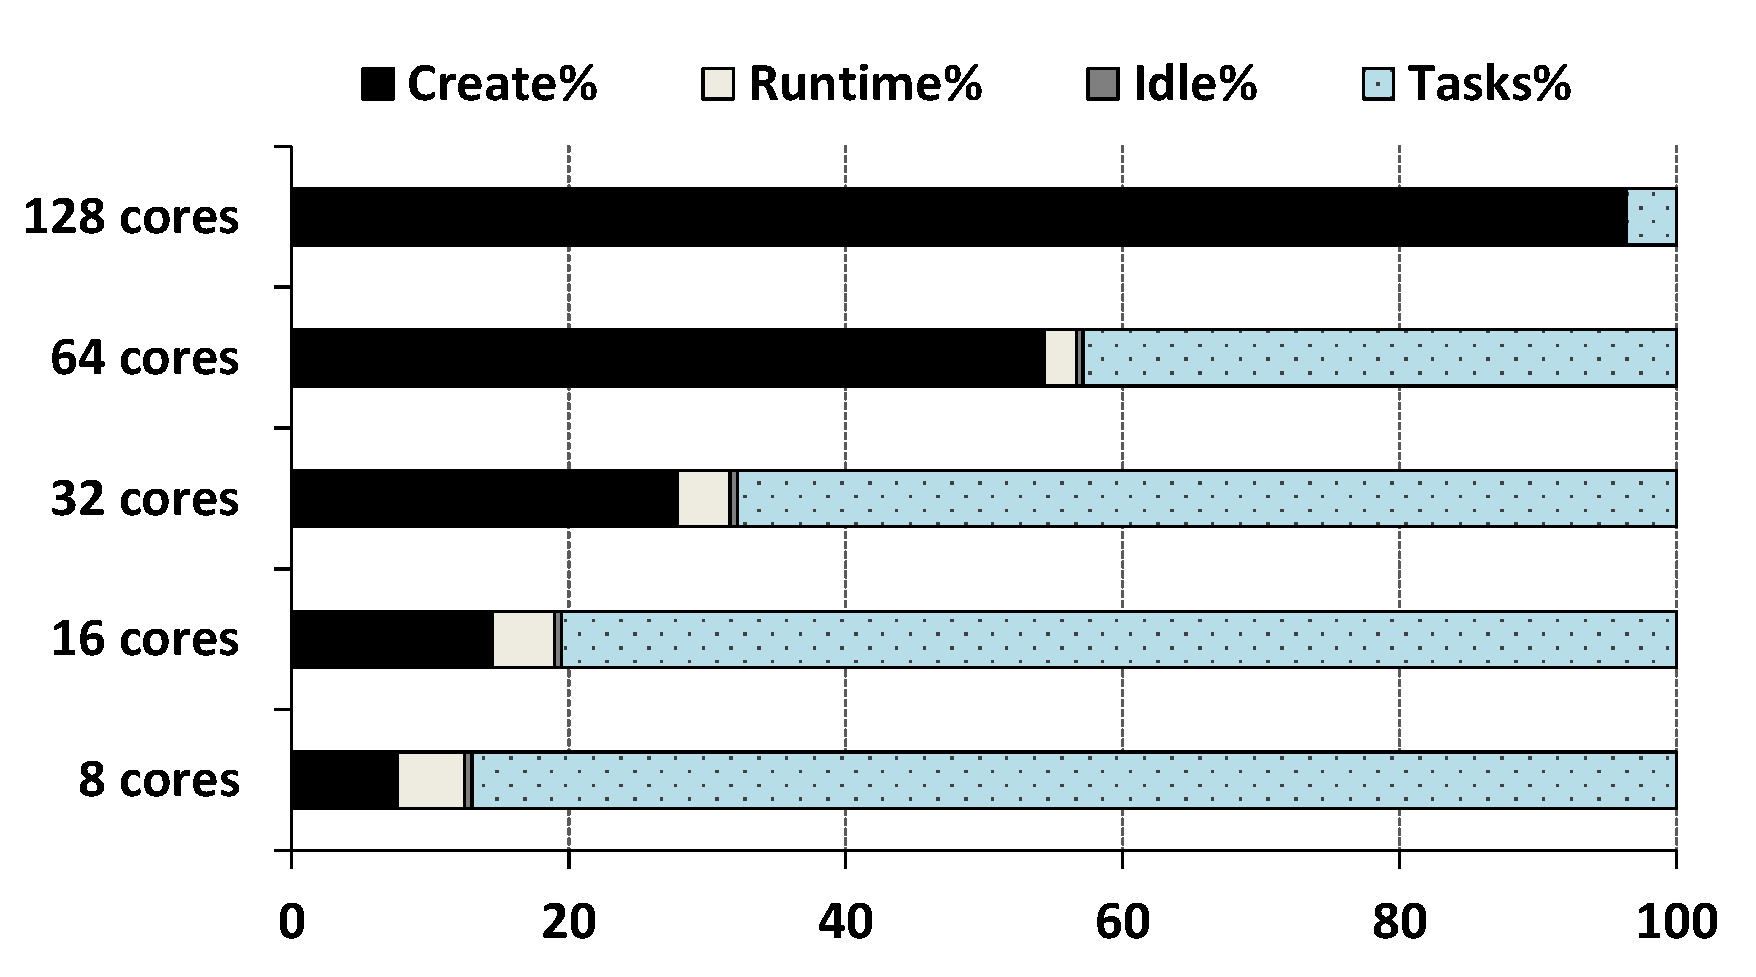
\includegraphics[width=.45\linewidth]{figures/master_thread.pdf}}
%	\subfigure[Figure 1]{\label{fig:sub1}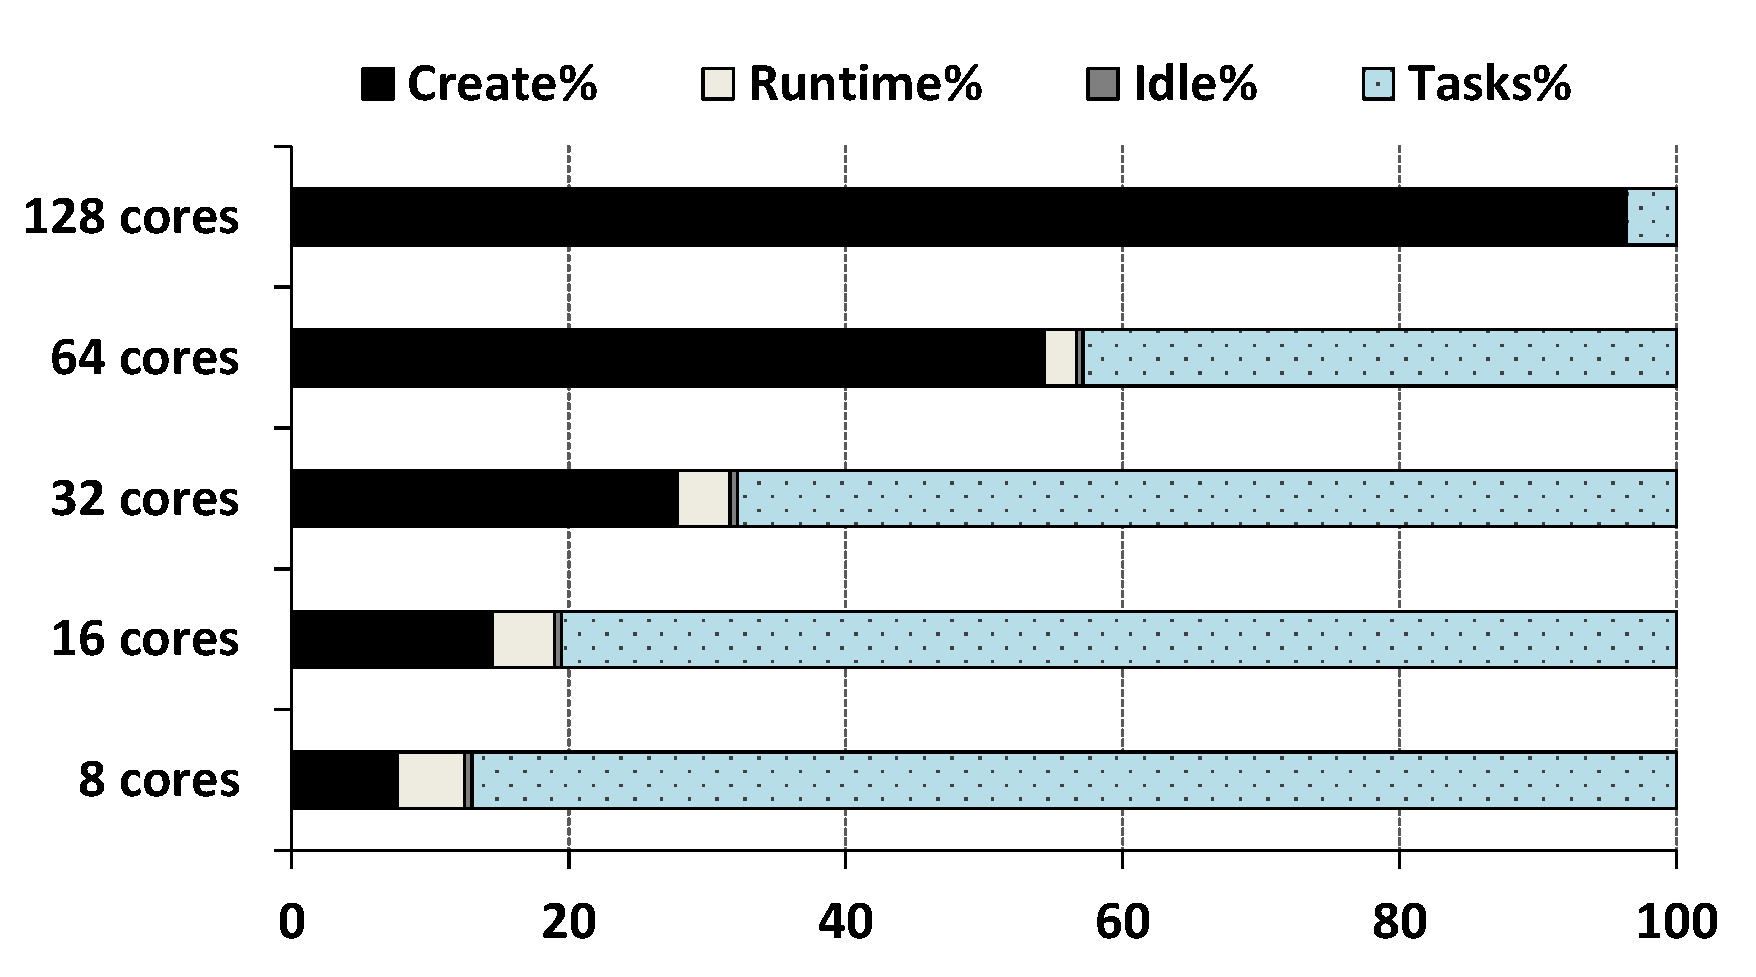
\includegraphics[width=.45\linewidth]{figures/master_thread.pdf}}
%	\caption{My caption}
%\end{figure}


\begin{figure}[t!]%
	\centering
	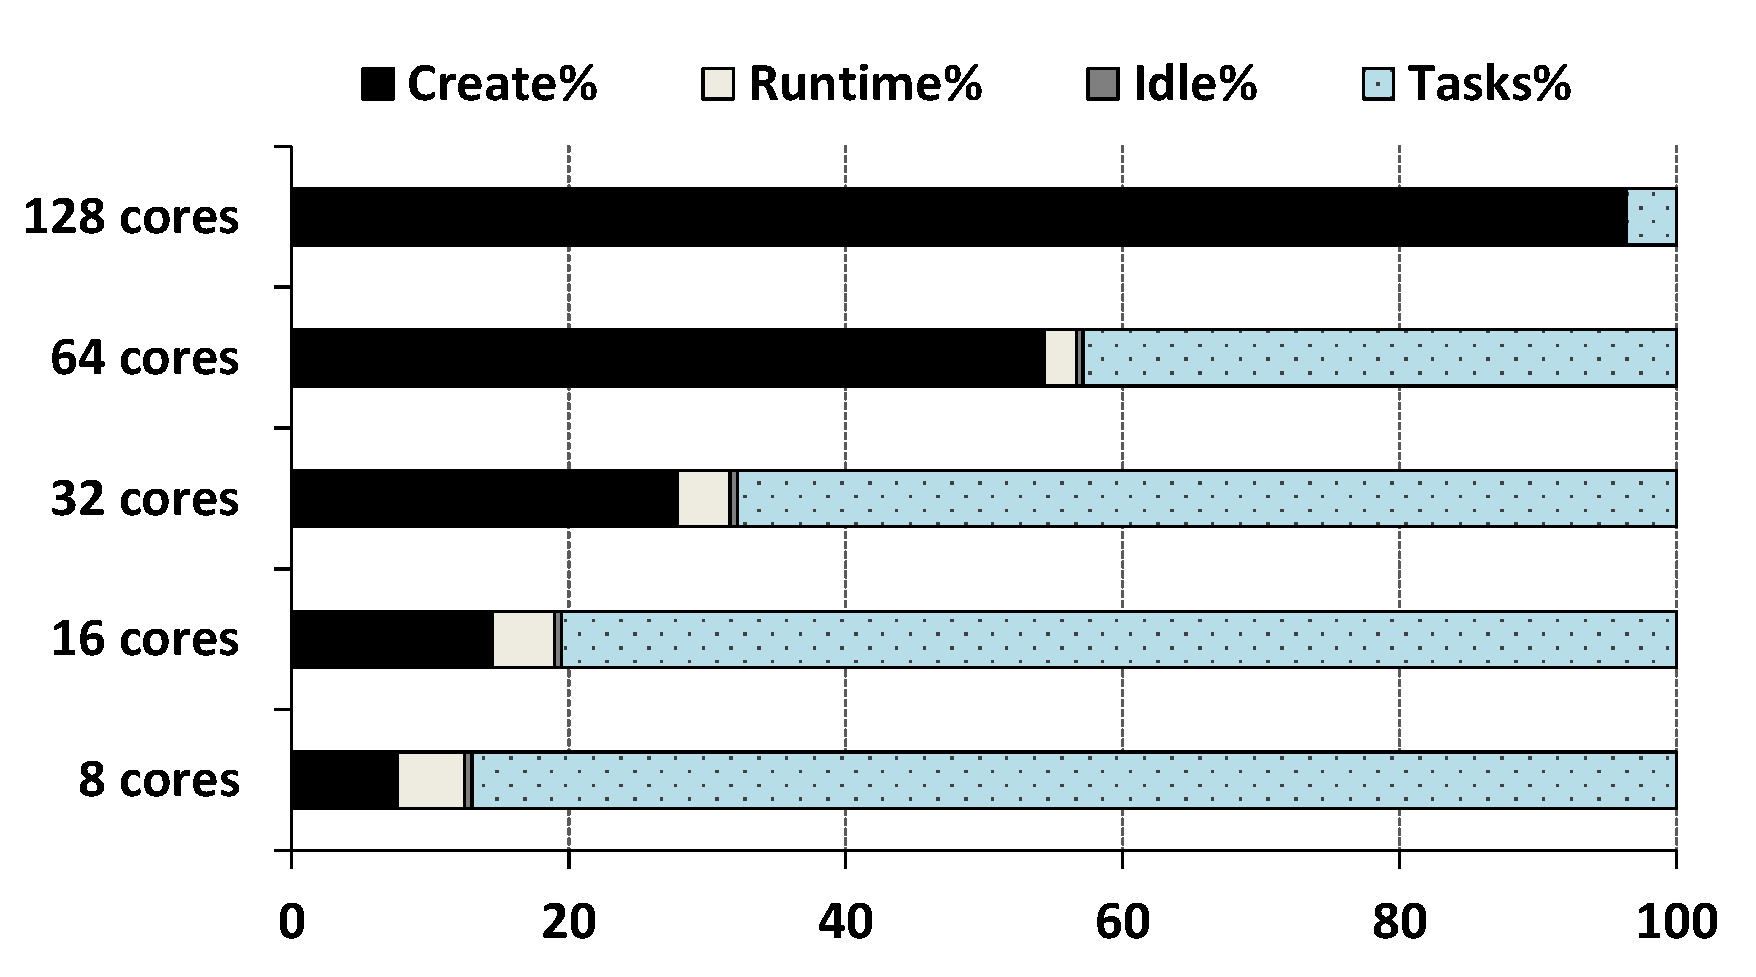
\includegraphics[width=0.75\columnwidth]{figures/master_thread.pdf}
	\caption{Master thread activity for Cholesky as we increase the number of cores.}
	%\caption{Performance improvements on a big.LITTLE processor with different $(F,N)$ configurations, where $F$ is the total number of big cores and $N$ the total number of cores. Results are normalized to running on four little cores with pinned Pthreads.}%
	\label{fig:master_thread}%
\end{figure}

Figure~\ref{fig:master_thread} shows the runtime activity of the master thread during the execution of the Cholesky{\footnote{Details about the benchmarks used are in Section~\ref{sec.background.applications}} benchmark on 8, 16, 32, 64 and 128 cores\footnote{The experimental set-up is explained in Section~\ref{sec.background.arm}}.
The execution time represented here is the wall clock time during the parallel region of the benchmark.
Each one of the series represents a different runtime overhead from the ones described above.
%\textit{Create} represents the \textit{Creation} step, 
%\textit{Runtime} refers to the \textit{Finish} step, \textit{Idle} shows the master thread's idle time and the \textit{Tasks} is the time spent on task execution. 
The percentage of time spent on task creation is increasing as we increase the number of cores.
This is because the creation overhead is invariant of core count: the more we reduce the application's execution time by adding resources the more important this step becomes in terms of execution time.
In contrast, the task execution time percentage is decreased as we increase the number of cores because the computational activity is being shared among more resources.
One way to reduce the task creation overhead is by introducing nested parallelism. 
In this programming technique, every worker thread is able to generate tasks thus the task creation is spread among cores and its overhead is reduced.
However, not all applications can be implemented with this parallelization technique and there are very few applications using this scheme.
\textit{Runtime} decreases as we increase the number of cores because this activity is also shared among the resources.
This is because this part of the runtime takes place once the tasks finish execution and new tasks are being scheduled. 
So the more the resources, the less the runtime activity per thread, therefore less activity for the master thread.
%\kc{explain that this is wall clock time. The \textit{Runtime} activity is actually the part of the master thread but also the worker threads are performing this activity while the Create is only within the master thread.}


Our motivation for this work is the bottleneck introduced by task creation as shown in Figure~\ref{fig:master_thread}.
Our runtime proposal decouples this piece of the runtime and accelerates it on a specialized hardware resulting in higher performance.



%%%%%%%%%%%%%%%%%%%
%%%%%%%%%%%%%%%%%%%
\section{Task Generation Express (TaskGenX)}
\label{sec.taskgenx.ram}
%We propose a hardware and software solution to overcome the performance bottleneck described in the previous section. 
%In our system we assume the existence of a specialized hardware that is responsible for the fast execution of the task creation. 
%To use such a hardware we need flexible software that manages to move the task creation to be executed there.

%The software that we employ uses a specialized queue for the task creation requests. 
%Each thread that is about to create a task instead of creating it, it inserts a task creation request in this queue. 
%The responsible hardware then reads the queue and executes the requests.

In this paper we propose a semi-centralized runtime system that dynamically separates the most computationally intensive parts of the runtime system and accelerates them on specialized hardware. 
To develop the {\proposal} we use the OpenMP programming model~\cite{OpenMP},~\cite{OpenMP4.0:Manual2015}.
The base of our implementation is the Nanos++ runtime system responsible for the parallel execution and it is used in this paper as a replacement of the entire OpenMP's default runtime.

Nanos++~\cite{nanos} is a distributed runtime system that uses dynamic scheduling.
As most task-based programming models, Nanos++ consists of the master and the worker threads.
The master thread is launching the parallel region and creates the tasks that have been defined by the programmer{\footnote{Nanos++ also supports nested parallelism so any of the worker threads can potentially create tasks. However the majority of the existing parallel applications are not implemented using nested parallelism.}}.
The scheduler of Nanos++ consists of a~\textit{ready queue} (\textit{TaskQ}) that is shared for reading and writing among threads and is used to keep the tasks that are ready for execution.
All threads have access to the \textit{TaskQ} and once they become available they try to pop a task from the \textit{TaskQ}.
When a thread finishes a task, it performs all the essential steps described in Section~\ref{sec.background} to keep the data dependency structures consistent.
Moreover, it pushes the tasks that become ready to the \textit{TaskQ}.

%We implement the Runtime Activity Manager ({\proposal}) on top of Nanos distributed runtime system that uses dynamic scheduling~\cite.


\subsection{Implementation}

{\proposal} relieves the master and worker threads from the intensive work of task creation by offloading it on the specialized hardware.
%{\proposal} assumes the existence of a specialized hardware that accelerates this part of the runtime.
Our runtime, apart from the master and the worker threads, introduces the Special Runtime Thread (SRT). 
When the runtime system starts, it creates the SRT and binds it to the task creation accelerator, keeping its thread identifier in order to manage the usage of it.
During runtime, the master and worker threads look for ready tasks in the task ready queue and execute them along with the runtime.
Instead of querying the ready queue for tasks, the SRT looks for runtime activity requests in the Runtime Requests Queue (\textit{RRQ}) and if there are requests, it executes them.

Figure~\ref{fig:communication} shows the communication infrastructure between threads within {\proposal}.
Our system maintains two queues; the Ready Task Queue (\textit{TaskQ}) and the Runtime Requests Queue (\textit{RRQ}).
The \textit{TaskQ} is used to keep the tasks that are ready for execution. 
The \textit{RRQ} is used to keep the pending runtime activity requests. 
The master and the worker threads can push and pop tasks to and from the \textit{TaskQ} and they can also add runtime activity to the \textit{RRQ}. 
The special runtime thread (SRT) pops runtime requests from the \textit{RRQ} and executes them on the accelerator.

When the master thread encounters a task clause in the application's code, after allocating the memory needed, it calls the \texttt{createTask} as shown in Listing~\ref{taskCreation} and described in Section~\ref{sec.background}. 
{\proposal} decouples the execution of \texttt{createTask} from the master thread. 
To do so, {\proposal} implements a wrapper function that is invoked instead of \texttt{createTask}.
In this function, the runtime system checks if the SRT is enabled; if not then the default behaviour takes place, that is, to perform the creation of the task.
If the SRT is enabled, a \textit{Create} request is generated and inserted in the \textit{RRQ}.
The \textit{Create} runtime request includes the appropriate info to execute the code described in Listing~\ref{taskCreation}.
That is, the dependence analysis data, the address of the allocated task, its parent and its arguments.



\begin{lstlisting}[float, emph={SRTloop}, caption={Pseudo-code for the SRT loop.},label=SRTloop]
void SRTloop() {
  while( true ) {   
    while(RRQ is not empty) 
      executeRequest( RRQ.pop() );
    if( runtime.SRTstop() ) break;
  }
  return; 
}  
\end{lstlisting}

While the master and worker threads are executing tasks, the SRT is looking for \textit{Create} requests in the \textit{RRQ} to execute.
Listing~\ref{SRTloop} shows the code that the SRT is executing until the end of the parallel execution.
The special runtime thread continuously checks whether there are requests in the \textit{RRQ} (line 3). 
If there is a pending creation request, the SRT calls the \texttt{executeRequest} (line 4), which extracts the appropriate task creation data from the creation request and performs the task creation by calling the \texttt{createTask} described in Listing~\ref{taskCreation}.
%executes the task submission and inserts the task in the TDG with a call to the \texttt{executeRequest} (line 4). 
When the parallel region is over, the runtime system informs the SRT to stop execution.
This is when the SRT exits and the execution finishes (line 5).

%\kc{communication:} To relieve the master and worker threads from the intensive runtime activity we use a simple queueing communication scheme that offloads the task submission on a specialized hardware.
%Whenever a thread encounters a task submission phase, instead of executing the submit call of the scheduler, it creates a runtime request and inserts it in the RRQ. 
%Concurrently, the SRT queries the RRQ for runtime requests and as long as there are requests available it executes them.
%Moreover, the SRT executes tasks whenever there are no requests for a long time to speedup the execution.


%\begin{figure}[tl]%
%	\centering
%	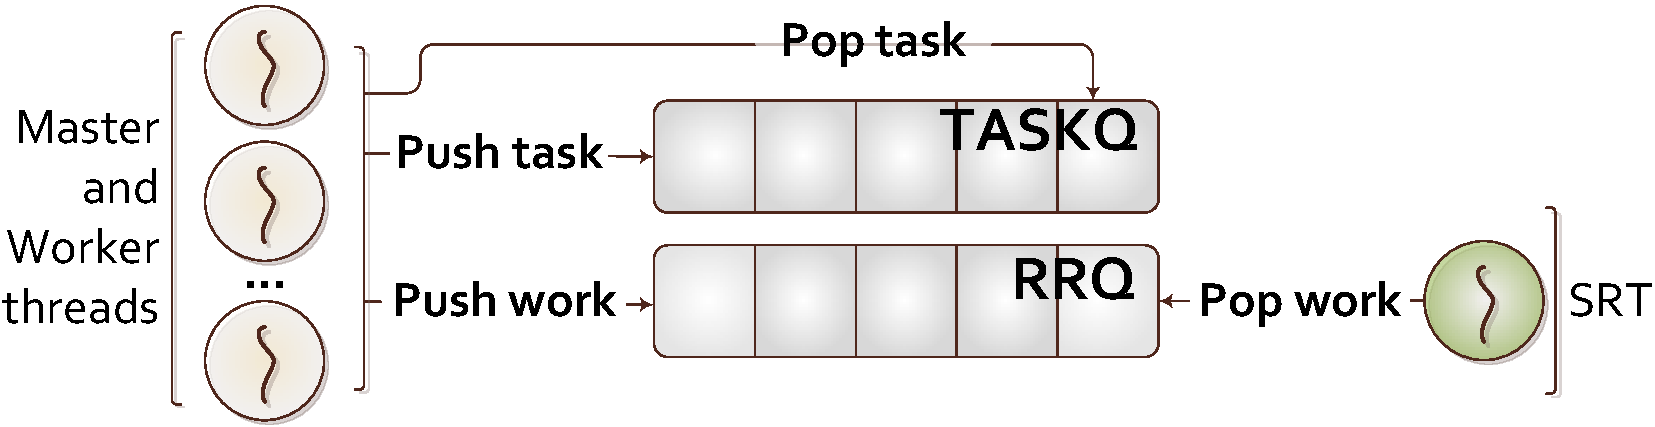
\includegraphics[width=0.4\columnwidth]{figures/communication2.pdf}
%	\caption{Communication mechanism between master/workers and SRT threads.}
%	\label{fig:communication}%
%	\vspace{-0.3cm}
%\end{figure}






%\section{Hardware requirements}}
%\label{sec:hw}
\subsection{Hardware Requirements}
\label{sec:hw_req}

%\begin{figure}[t]%
%	\centering
%	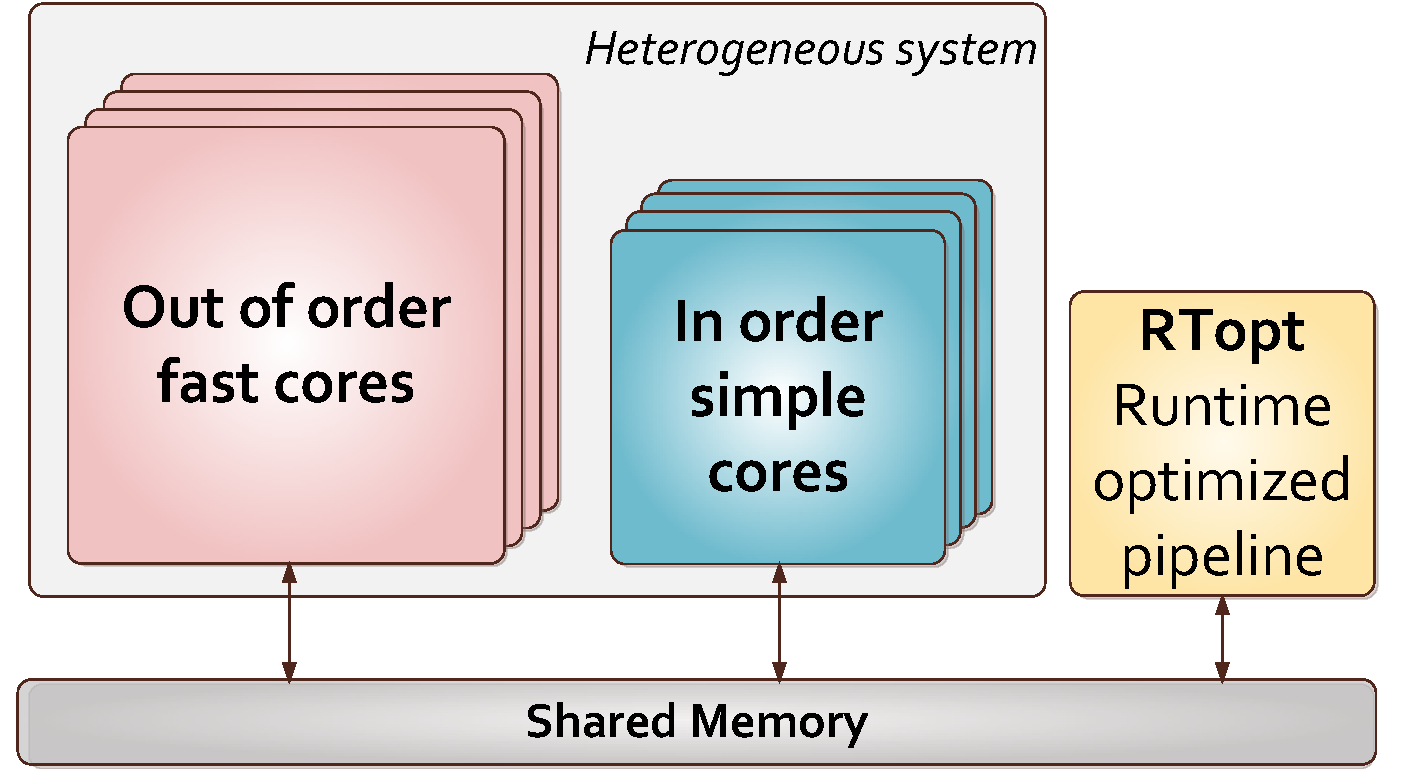
\includegraphics[width=0.6\columnwidth]{figures/hw_fig.pdf}
%	\caption{SoC architecture including three types of cores: out of order, in-order and RTopt.}
%	\label{fig:hw}%
%	\vspace{-0.3cm}
%\end{figure}
As described in the previous section, {\proposal} assumes the existence of specialized hardware that accelerates the task creation step. 
The goal of this paper is not to propose a detailed micro-architecture of the specialized hardware; instead we sketch the high-level hardware requirements for the {\proposal} set-up, in the hope to be an insightful and useful influence for hardware designers.
The SRT is bound to the task creation accelerator and executes the requests in the RRQ. 
Previous studies have proposed custom accelerators for the runtime activity~\cite{TaskSS, Xubin, Nexus, Swarm, TMU, Carbon}. 
These proposals significantly accelerate (up to three orders of magnitude) different bottlenecks of the runtime system\footnote{Section~\ref{sec:related} further describes these proposals.}. 
These special purpose designs can only execute runtime system activity.

%\begin{figure}[t!]%
%	\centering
%	\subfloat[Communication mechanism between master/workers and SRT threads.]{\label{fig:communication}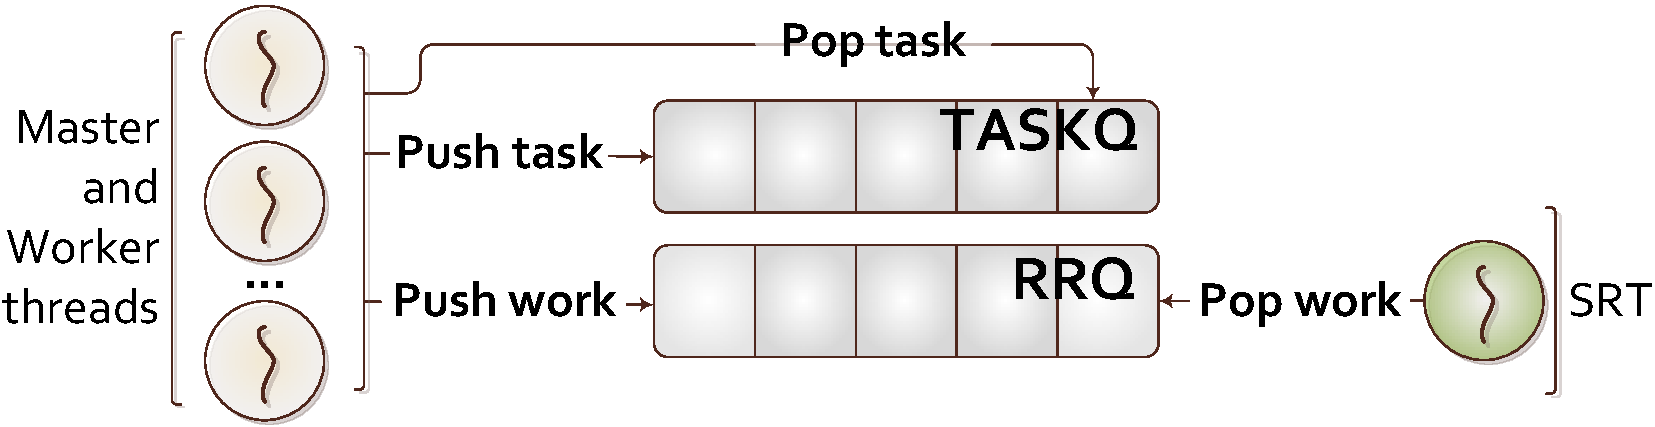
\includegraphics[width=0.5\columnwidth]{figures/communication2.pdf}} \hspace{0.2cm}
%	\subfloat[SoC architecture including three types of cores: out of order, in-order and RTopt.]{\label{fig:hw}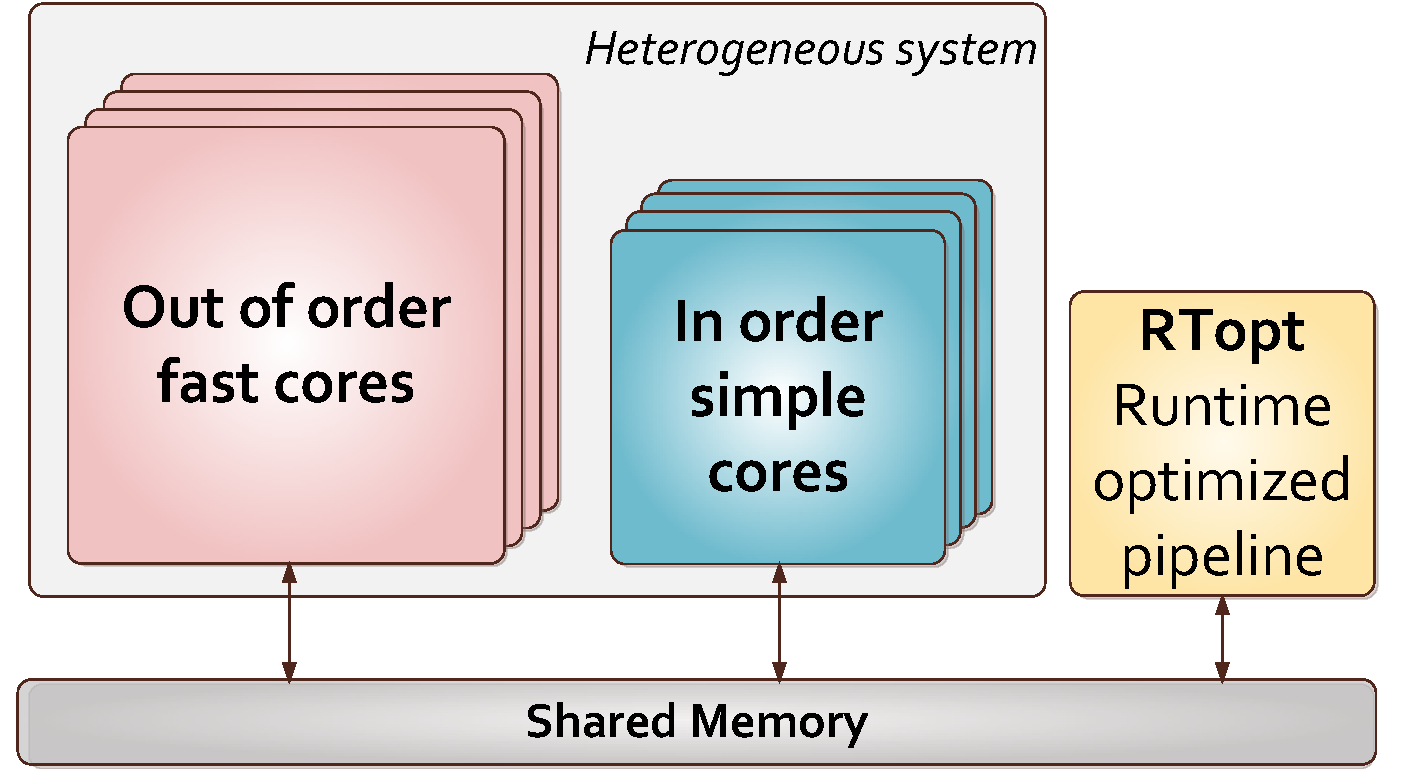
\includegraphics[width=0.4\linewidth]{figures/hw_fig.pdf}}
%	\caption{}
%\end{figure}

\begin{figure}[t!]%
	\centering
	
	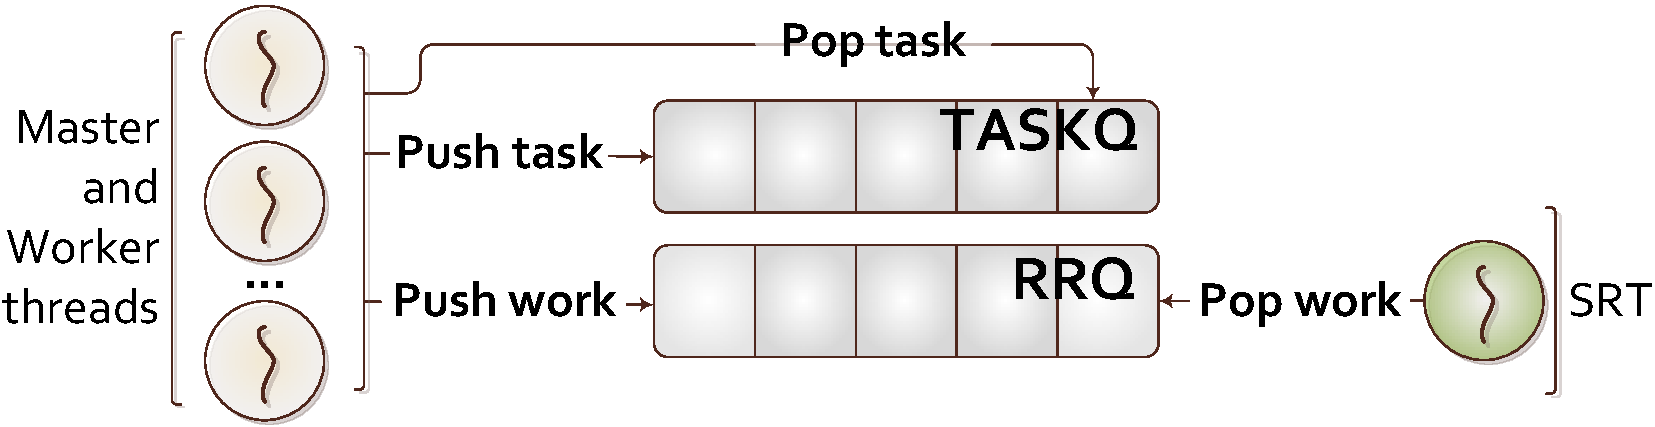
\includegraphics[width=0.9\textwidth]{figures/communication2.pdf}
	\caption{Communication mechanism between master/workers and SRT threads.}
	\label{fig:communication}
\end{figure}
	
As an alternative, in our envisioned architecture we propose to have a general purpose core that has been optimized to run the runtime system activity more efficiently. 
The runtime optimized (RTopt) core can be combined with both homogeneous or heterogeneous systems and accelerate the runtime activity.
Figure~\ref{fig:hw} shows the envisioned architecture when RTopt is combined with an asymmetric heterogeneous system.
%Figure~\ref{fig:hw} shows the envisioned asymmetric multi-core architecture with different core types. 
This architecture has three core types that consist of simple in-order cores, fast out-of-order cores and an RTopt core for the SRT. 
RTopt can optimize its architecture, having a different cache hierarchy, pipeline configuration and specialized hardware structures to hold and process the SRT. 
As a result, the RTopt executes the SRT much faster than the other cores. 
The RTopt can also execute tasks, but will achieve limited performance compared to the other cores as its hardware structures have been optimized for a specific software (the SRT).
\begin{figure}[t!]
	\centering
	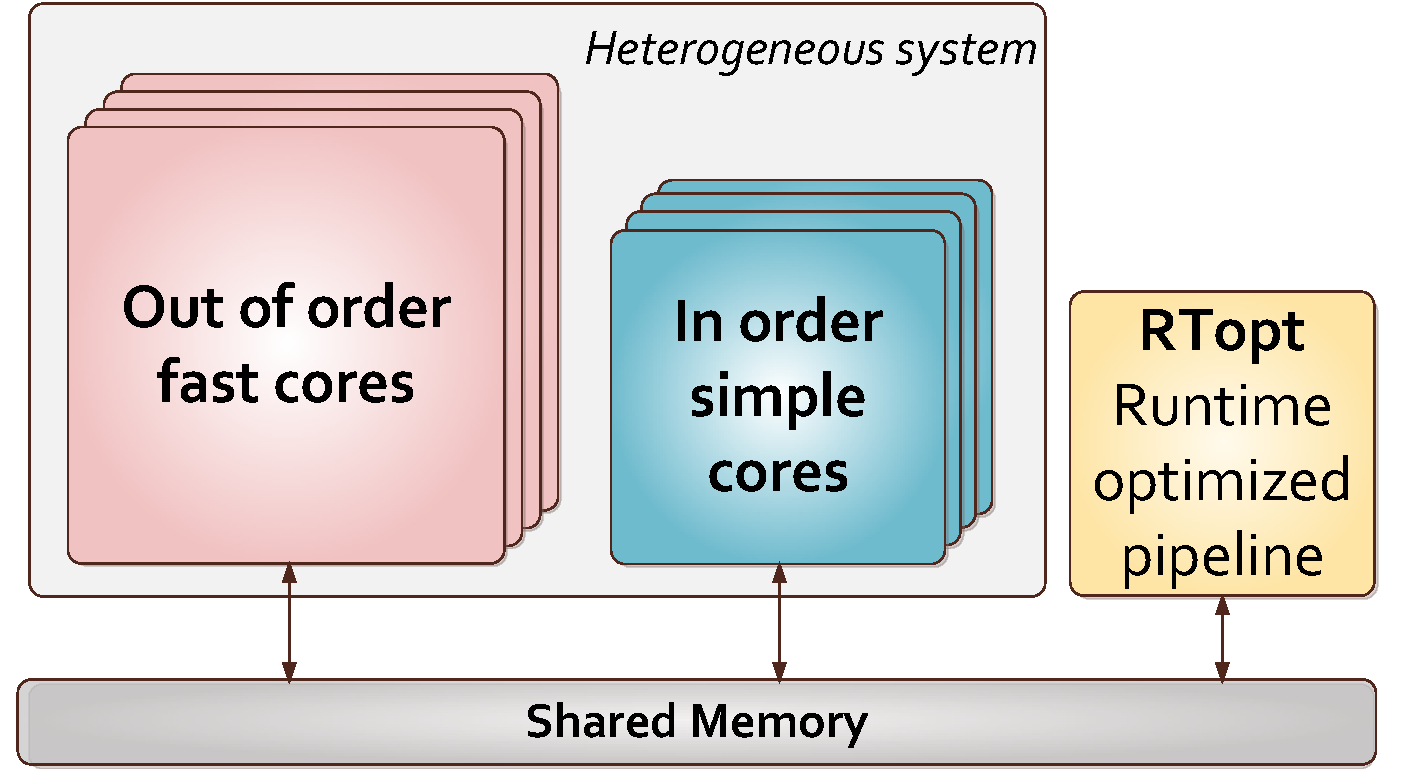
\includegraphics[width=0.6\textwidth]{figures/hw_fig.pdf}
	\caption{SoC architecture including three types of cores: out of order, in-order and RTopt.}
	\label{fig:hw}
\end{figure}
To evaluate our approach we study the requirements of the RTopt in order to provide enough performance for {\proposal}.
Based on the analysis by Etsion et al.~\cite{TaskSS}, there is a certain \textit{task decode rate} that leads to optimal utilization of the multi-core system.
This rule can be applied in the case of {\proposal} for the \textit{task creation rate}, i.e., the frequency of task generation of the runtime system.
If the \textit{task creation rate} is higher than the \textit{task execution rate}, then for a highly parallel application the resources will always have tasks to execute and they will not remain idle.
To achieve a high \textit{task creation rate}, we can accelerate the task creation cost.
Equation~\ref{eq.create} shows the maximum optimal task creation cost, $C_{opt}(x)$ in order to keep $x$ cores busy, without starving due to task creation.

%\begingroup\makeatletter\def\f@size{9}\check@mathfonts
\begin{equation}
  \text{$C_{opt}(x) = avg.\ task\ duration / x$ }
\label{eq.create}
\end{equation}
%\endgroup

If $C_{gp}$ is the cost of task creation when it is performed on a general purpose core, then the RTopt has to achieve a speedup of $r = C_{gp}/C_{opt}(x)$ to achieve full utilization of the system. 
Section~\ref{sec:experimental:simulation} performs an analysis based on these requirements for the evaluated applications. 
As we will see in Section~\ref{sec:experimental:simulation}, a modest and implementable value of $r=16\times$ is enough to significantly accelerate execution on a 512-core system.

Finally, if {\proposal} executes on a regular processor without the RTopt core, the SRT is bound to a regular core without any further modification. In this scenario, applications will not significantly benefit from having a separate SRT.




%%%%%%%%%%%%%%%%%%%
%%%%%%%%%%%%%%%%%%%

\begin{table*}[t]
\begin{center}
\caption{Evaluated benchmarks and relevant characteristics}
\label{tab.apps}
\resizebox{\textwidth}{!}{%
\begin{tabular}{|c|c|c|c|c|c|c|c|c|c|}
\hline
\multirow{3}{*}{\parbox{13mm}{\centering Application}} & 
\multirow{3}{*}{Problem size} & 
\multirow{3}{*}{\parbox{10mm}{\centering \#Tasks}} & 
\multirow{3}{*}{\parbox{17mm}{\centering Avg task CPU cycles (thousands)}} & 
\multicolumn{3}{|c|}{\parbox{22mm}{\centering Per task overheads (CPU cycles)}} & & &\\
\cline{5-7}
& & & & \multirow{2}{*}{\parbox{10mm}{\centering Create}} & \multirow{2}{*}{\parbox{9mm}{\centering All}} & \multirow{2}{*}{\parbox{11mm}{\centering Deps + Sched}} & \multirow{2}{*}{\parbox{15mm}{\centering Measured perf. ratio}} &
{\parbox{10mm}{\centering $r$}} &
\multirow{2}{*}{\parbox{11mm}{\centering Parallel model}} \\
& & & & & & & & & \\ %\hhline{~~~~~~}
\hline

\multirow{2}{*}{\parbox{18mm}{\centering Cholesky factorization}} & 
32K 256 & 357\,762  & 753 & 15221 &  73286 &  58065 &  \multirow{2}{*}{\parbox{9mm}{\centering 3.5}} & 10.34 & \multirow{2}{*}{\parbox{17mm}{\centering dependencies}}\\                                              & 32K 128 & 2829058 & 110 & 17992 &  58820 &  40828 & & 83.74 &\\
%& 32$\times$32 blocks of 512$\times$512 floats & 5984 & & 1\,551\,322 & 104.76 &  238.02 &  194.28  & \\ 
\hline{}
\multirow{2}{*}{\parbox{18mm}{\centering QR factorization}} & 16K 512 & 11\,442 & 518\,570  & 17595 & 63008 &   45413 & \multirow{2}{*}{\parbox{9mm}{\centering 6.8}} & 0.01 &\multirow{2}{*}{\parbox{17mm}{\centering dependencies}}\\
&  16K 128 & 707\,265 & 3\,558 & 21642 & 60777 & 39135 & & 3.11 &\\
\hline
Blackscholes & native & 488\,202 & 348  &   29141  &  85438 &  56297 & 2.3 & 42.87 & data-parallel \\
\hline
Bodytrack & native & 329\,123 & 383 &  9\,505 &  18979 & 9474 & 4.2 & 12.70 & pipeline \\ 
%Heat diffusion & Heat &  &  &  &  &  & \\ 
\hline
Canneal & native & 3\,072\,002 & 67 & 25781 & 50094 &  24313 & 2.0 & 197.01 & unstructured \\
\hline
Dedup & native & 20\,248 & 1\,532 & 1294 & 9647 &  8353 & 2.7 & 0.43 & pipeline \\
\hline 
Ferret & native$\times$2 & 84\,002 & 29\,088 & 38913 & 98457 &  59544 & 3.6 & 0.68 & pipeline \\
\hline
Fluidanimate & native & 128\,502 & 16\,734 & 30210 & 94079 &  64079 & 3.3 & 0.91 & data-parallel \\
\hline
Streamcluster & native & 3\,184\,654 & 161 & 6892 & 13693 &  6801 & 3.5 & 21.91 & data-parallel \\
\hline
\end{tabular}}
\end{center}
\vspace{-0.4cm}
\end{table*}

\subsection{Applications}
%\begin{itemize}
%\item Blackscholes
%\item Cholesky
%\item Canneal
%\item Fluidanimate
%\item QR Factorization
%\item Bodytrack
%\item Streamcluster
%\end{itemize}
Table~\ref{tab.apps} shows the evaluated applications, the input sizes used, and their characteristics. 
All applications are implemented using the OpenMP programming model~\cite{OpenMP4.0:Manual2015}. 
We obtain Cholesky and QR from the BAR repository~\cite{BAR} and we use the implementations of the rest of the benchmarks from the PARSECSs suite~\cite{Chasapis:TACO2016}.
More information about these applications can be found in~\cite{Chasapis:TACO2016} and~\cite{Chronaki:ICS2015}.
As the number of cores in SoCs is increasing, so does the need of available task parallelism~\cite{Sanchez:2010}. 
We choose the input sizes of the applications so that they create enough fine-grained tasks to feed up to 512 cores.
The number of tasks per application and input as well as the average per-task CPU cycles can be found on Table~\ref{tab.apps}.





\subsection{Simulation}
\label{TaskGenX:experimental:simulation}
To evaluate TaskGenX we make use of the TaskSim trace-driven simulator~\cite{AbstrLevels_TACO12,MUSA} as explained in Section~\ref{sec.background.simulation}. 

We evaluate both symmetric and asymmetric systes with the number of cores varying from 8 to 512.
To set the correct performance ratio between big and little cores for the asymetric systems, we measure the sequential execution time of each application on a real ARM big.LITTLE platform when running on a little and on a big core. 
We use the Hardkernel Odroid~XU3 board that includes a Samsung Exynos 5422 chip with ARM big.LITTLE.
The big cores run at 1.6GHz and the little cores at 800MHz.
Table~\ref{tab.apps} shows the measured performance ratio for each case.
The average performance ratio among our 11 workloads is 3.8.
Thus in the specification of the asymmetric systems we use as performance ratio the value 4.

We modify TaskSim so that it features one extra hardware accelerator (per multi-core) responsible for the fast task creation (the RTopt).
Apart from the task duration time, our modified simulator tracks the duration of the runtime overheads.
These overheads include: (a) task creation, (b) dependencies resolution, and (c) scheduling.
The RTopt core is optimized to execute task creation faster than the general purpose cores; 
to determine how much faster a task creation job is executed we use the analysis performed in Section~\ref{sec:hw_req}.

Using Equation~\ref{eq.create}, we compute the $C_{opt}(x)$ for each application according to their average task CPU cycles from Table~\ref{tab.apps} for $x=512$ cores.
$C_{gp}$ is the cost of task creation when it is performed on a general purpose core, namely the \textit{Create} column shown on Table~\ref{tab.apps}.
To have optimal results for each application on systems up to 512 cores, $C_{gp}$ needs to be reduced to $C_{opt}(512)$.
Thus the specialized hardware accelerator needs to perform task creation with a ratio $r = C_{gp}/C_{opt}(512) \times$ faster than a general purpose core.

We compute $r$ for each application shown on Table~\ref{tab.apps}. We observe that for the applications with a large number of per-task CPU cycles and relatively small \textit{Create} cycles (QR512, Dedup, Ferret, Fluidanimate), $r$ is very close to zero, meaning that the task creation cost ($C_{gp}$) is already small enough for optimal task creation without the need of a faster hardware accelerator.
For the rest of the applications, more powerful hardware is needed.
For these applications $r$ ranges from 3$\times$ to 197$\times$.
Comparing $r$ to the measured performance ratio of each application we can see that in most cases accelerating the task creation on a big core would not be sufficient for achieving higher task creation rate.
In our experimental evaluation we accelerate task creation in the RTopt and we use the ratio of 16$\times$ which is a relatively small value within this range that we consider realistic to implement in hardware.
%Contrarily, if RTopt is assigned a task to execute, we assume that it executes it 4$\times$ slower than a general purpose in-order core.
The results obtained show the average results among three different traces for each application-input.

%%%%%%%%%%%%%%%%%%%
%%%%%%%%%%%%%%%%%%%
\section{Evaluation}
\label{sec.taskgenx.evaluation}
\subsection{Methodology}
\label{sec.taskgenx.methodology}
\begin{table*}[t]
	\scriptsize
	\begin{center}
		\caption{Evaluated benchmarks and relevant characteristics}
		\label{tab.apps}
		\resizebox{\textwidth}{!}{%
			\begin{tabular}{|c|c|c|c|c|c|c|c|c|}
				\hline
				\multirow{3}{*}{\parbox{15mm}{\centering Application}} & 
				\multirow{3}{*}{Problem size} & 
				\multirow{3}{*}{\parbox{10mm}{\centering \#Tasks}} & 
				\multirow{3}{*}{\parbox{17mm}{\centering Avg task CPU cycles (thousands)}} & 
				\multicolumn{3}{|c|}{\parbox{22mm}{\centering Per task overheads (CPU cycles)}} & & \\
				\cline{5-7}
				& & & & \multirow{2}{*}{\parbox{10mm}{\centering Create}} & \multirow{2}{*}{\parbox{9mm}{\centering All}} & \multirow{2}{*}{\parbox{11mm}{\centering Deps + Sched}} & \multirow{2}{*}{\parbox{15mm}{\centering Measured perf. ratio}} &
				\multirow{2}{*}{\parbox{10mm}{\centering $r$}} \\
				& & & & & & & &  \\ %\hhline{~~~~~~}
				\hline
				
				\multirow{2}{*}{\parbox{20mm}{\centering Cholesky factorization}} & 32K 256 & 357\,762  & 753 & 15221 &  73286 &  58065 &  \multirow{2}{*}{\parbox{9mm}{\centering 3.5}} & 10.34 \\                                              
				& 32K 128 & 2829058 & 110 & 17992 &  58820 &  40828 & & 83.74 \\
				%& 32$\times$32 blocks of 512$\times$512 floats & 5984 & & 1\,551\,322 & 104.76 &  238.02 &  194.28  & \\ 
				\hline{}
				\multirow{2}{*}{\parbox{18mm}{\centering QR factorization}} & 16K 512 & 11\,442 & 518\,570  & 17595 & 63008 &   45413 & \multirow{2}{*}{\parbox{9mm}{\centering 6.8}} & 0.01 \\
				&  16K 128 & 707\,265 & 3\,558 & 21642 & 60777 & 39135 & & 3.11 \\
				\hline
				Blackscholes & native & 488\,202 & 348  &   29141  &  85438 &  56297 & 2.3 & 42.87   \\
				\hline
				Bodytrack & native & 329\,123 & 383 &  9\,505 &  18979 & 9474 & 4.2 & 12.70   \\ 
				%Heat diffusion & Heat &  &  &  &  &  & \\ 
				\hline
				Canneal & native & 3\,072\,002 & 67 & 25781 & 50094 &  24313 & 2.0 & 197.01   \\
				\hline
				Dedup & native & 20\,248 & 1\,532 & 1294 & 9647 &  8353 & 2.7 & 0.43   \\
				\hline 
				Ferret & native$\times$2 & 84\,002 & 29\,088 & 38913 & 98457 &  59544 & 3.6 & 0.68   \\
				\hline
				Fluidanimate & native & 128\,502 & 16\,734 & 30210 & 94079 &  64079 & 3.3 & 0.91   \\
				\hline
				Streamcluster & native & 3\,184\,654 & 161 & 6892 & 13693 &  6801 & 3.5 & 21.91   \\
				\hline
		\end{tabular}}
	\end{center}
	\vspace{-0.4cm}
\end{table*}

\subsubsection{Applications}
%\begin{itemize}
%\item Blackscholes
%\item Cholesky
%\item Canneal
%\item Fluidanimate
%\item QR Factorization
%\item Bodytrack
%\item Streamcluster
%\end{itemize}
Table~\ref{tab.apps} shows the evaluated applications, the input sizes used, and their characteristics. 
All applications are implemented using the OpenMP programming model~\cite{OpenMP4.0:Manual2015}. 
We obtain Cholesky and QR from the BAR repository~\cite{BAR} and we use the implementations of the rest of the benchmarks from the PARSECSs suite~\cite{Chasapis:TACO2016}.
More information about these applications can be found in~\cite{Chasapis:TACO2016} and~\cite{Chronaki:ICS2015}.
As the number of cores in SoCs is increasing, so does the need of available task parallelism~\cite{Sanchez:2010}. 
We choose the input sizes of the applications so that they create enough fine-grained tasks to feed up to 512 cores.
The number of tasks per application and input as well as the average per-task CPU cycles can be found on Table~\ref{tab.apps}.





\subsubsection{Simulation}
\label{sec:experimental:simulation}
To evaluate {\proposal} we make use of the trace-driven TaskSim simulator~\cite{AbstrLevels_TACO12,MUSA} which is described in section~\ref{sec.background.simulation}. 
%Added in the background section:
%TaskSim is a trace driven simulator, that supports the specification of homogeneous or heterogeneous systems with many cores. 
%The tracing overhead of the simulator is less than 10\% and the simulation is accurate as long as there is no contention in the shared memory resources on a real system~\cite{MUSA}.
%By default, TaskSim allows the specification of the amount of cores and supports up to two core types in the case of heterogeneous asymmetric systems. 
%This is done by specifying the number of cores of each type and their difference in performance between the different types (performance ratio) in the TaskSim configuration file.

We evaluate the effectiveness of TaskGenX on both symmetric and asymmetric platforms with the number of cores varying from 8 to 512.
In the case of asymmetric systems, we simulate the behavior of an ARM big.LITTLE architecture~\cite{ARM}.
To set the correct performance ratio between big and little cores, we measure the sequential execution time of each application on a real ARM big.LITTLE platform when running on a little and on a big core. 
We use the Hardkernel Odroid~XU3 board that includes a Samsung Exynos 5422 chip with ARM big.LITTLE.
The big cores run at 1.6GHz and the little cores at 800MHz.
%We compare its performance when they run on a little and on a big core.
Table~\ref{tab.apps} shows the measured performance ratio for each case.
The average performance ratio among our 11 workloads is 3.8.
Thus in the specification of the asymmetric systems we use as performance ratio the value 4.

%Added in the background:
%To simulate our approaches using TaskSim we first run each application/input in the TaskSim trace generation mode.
%This mode enables the online tracking of task duration and synchronization overheads and stores them in a trace file. 
%To perform the simulation, TaskSim uses the information stored in the trace file and executes the application by providing this information to the runtime system.
%For our experiments we generate three trace files for each application/input combination on a Genuine Intel 16-core machine running at 2.60GHz.

For the needs of this hardware-software co-design, we modify TaskSim so that it features one extra hardware accelerator (per multi-core) responsible for the fast task creation (the RTopt).
Apart from the task duration time, our modified simulator tracks the duration of the runtime overheads.
These overheads include: (a) task creation, (b) dependencies resolution, and (c) scheduling.
The RTopt core is optimized to execute task creation faster than the general purpose cores; 
to determine how much faster a task creation job is executed we use the analysis performed in Section~\ref{sec:hw_req}.

Using Equation~\ref{eq.create}, we compute the $C_{opt}(x)$ for each application according to their average task CPU cycles from Table~\ref{tab.apps} for $x=512$ cores.
$C_{gp}$ is the cost of task creation when it is performed on a general purpose core, namely the \textit{Create} column shown on Table~\ref{tab.apps}.
To have optimal results for each application on systems up to 512 cores, $C_{gp}$ needs to be reduced to $C_{opt}(512)$.
Thus the specialized hardware accelerator needs to perform task creation with a ratio $r = C_{gp}/C_{opt}(512) \times$ faster than a general purpose core.

We compute $r$ for each application shown on Table~\ref{tab.apps}. We observe that for the applications with a large number of per-task CPU cycles and relatively small \textit{Create} cycles (QR512, Dedup, Ferret, Fluidanimate), $r$ is very close to zero, meaning that the task creation cost ($C_{gp}$) is already small enough for optimal task creation without the need of a faster hardware accelerator.
For the rest of the applications, more powerful hardware is needed.
For these applications $r$ ranges from 3$\times$ to 197$\times$.
Comparing $r$ to the measured performance ratio of each application we can see that in most cases accelerating the task creation on a big core would not be sufficient for achieving higher task creation rate.
In our experimental evaluation we accelerate task creation in the RTopt and we use the ratio of 16$\times$ which is a relatively small value within this range that we consider realistic to implement in hardware.
%Contrarily, if RTopt is assigned a task to execute, we assume that it executes it 4$\times$ slower than a general purpose in-order core.
The results obtained show the average results among three different traces for each application-input.

\subsection{Homogeneous Multicore Systems}
%\begin{figure}[t]%
%    \label{fig:speedup_homo}
%	\centering
%	%\begin{subfigure}
%	\subfloat [] 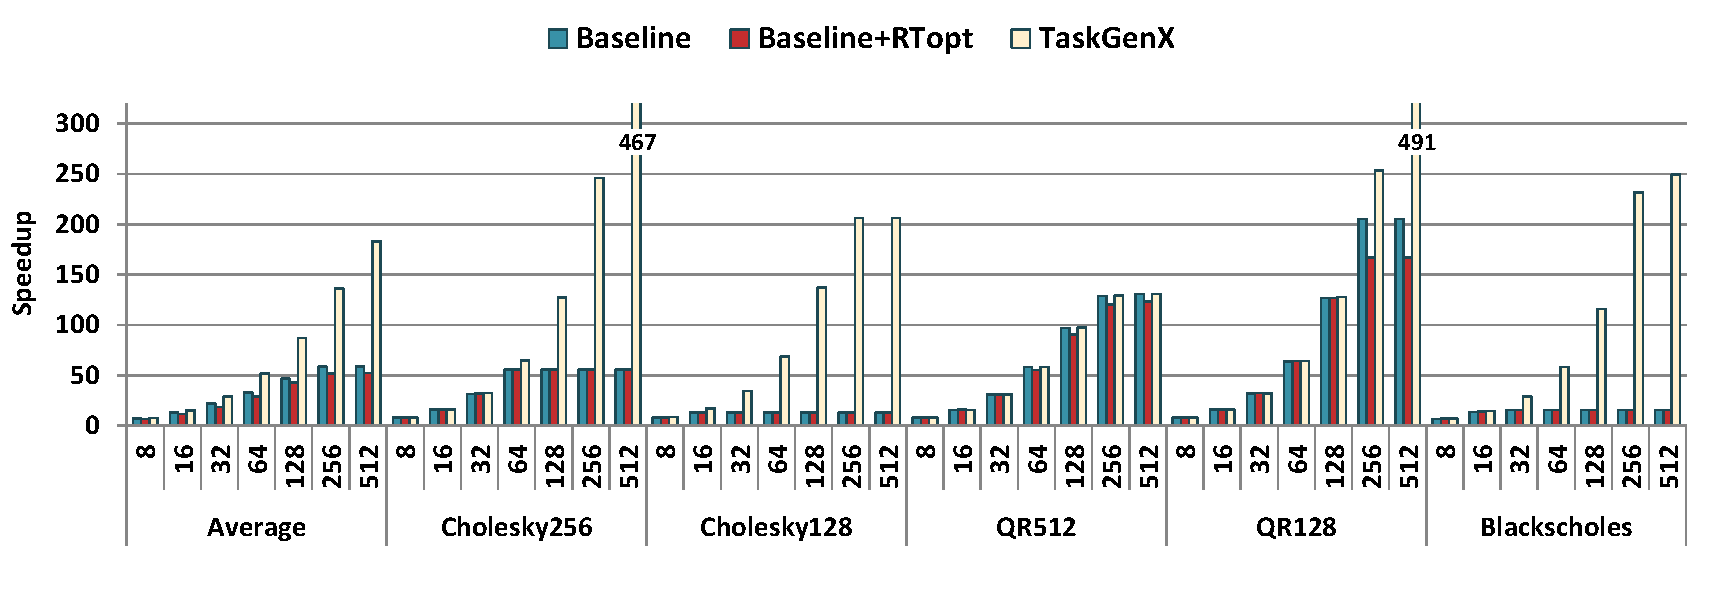
\includegraphics[width=1.0\textwidth]{figures/speedup_homo.pdf}
%	%\caption{test}
%	%\end{subfigure}
%	%\begin{subfigure}
%	\subfloat [] 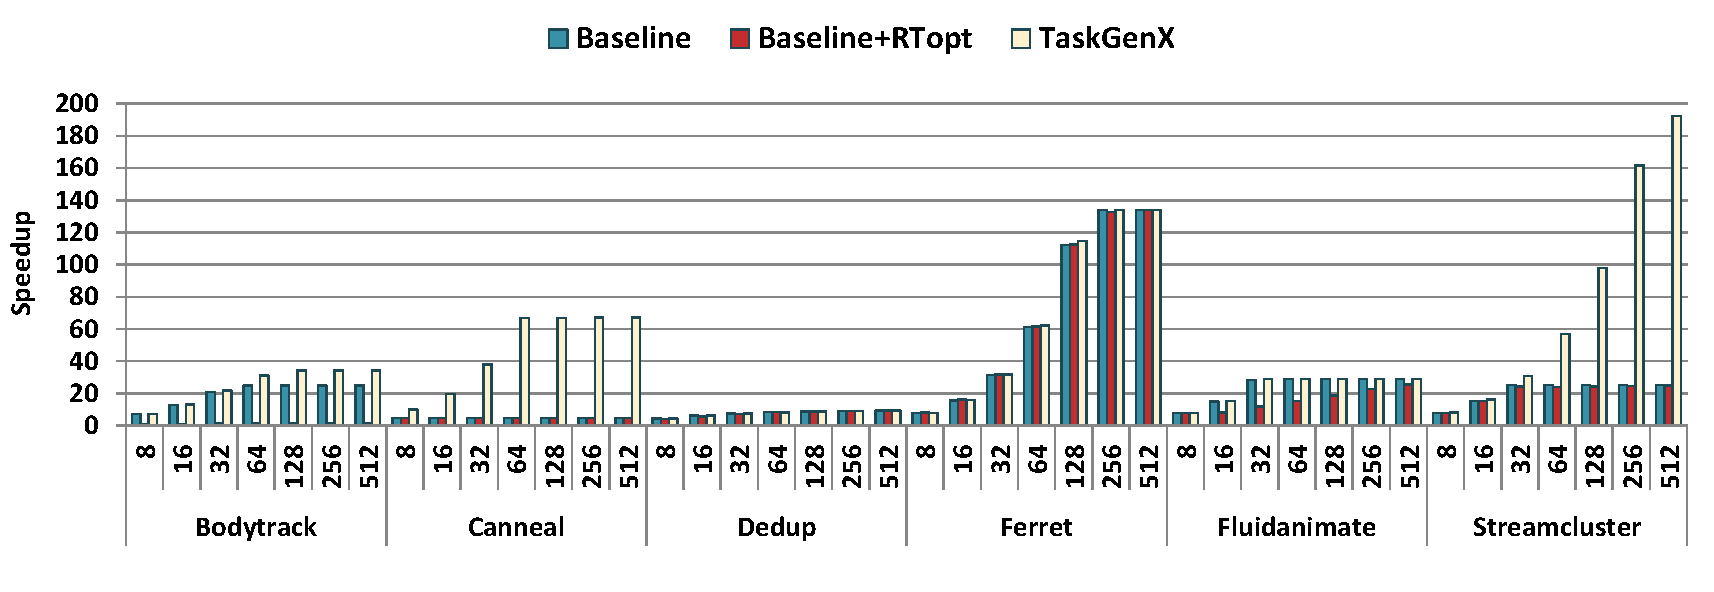
\includegraphics[width=1.0\textwidth]{figures/speedup_homo2.pdf}
%	%\end{subfigure}
%	\vspace{-0.5cm}
%	\caption{Communication mechanism between master/workers and SRT threads.}
%	\vspace{-0.3cm}
%\end{figure}

\begin{figure}[t]%
	\centering
	\subfloat[]{\label{fig:speedup_homo1}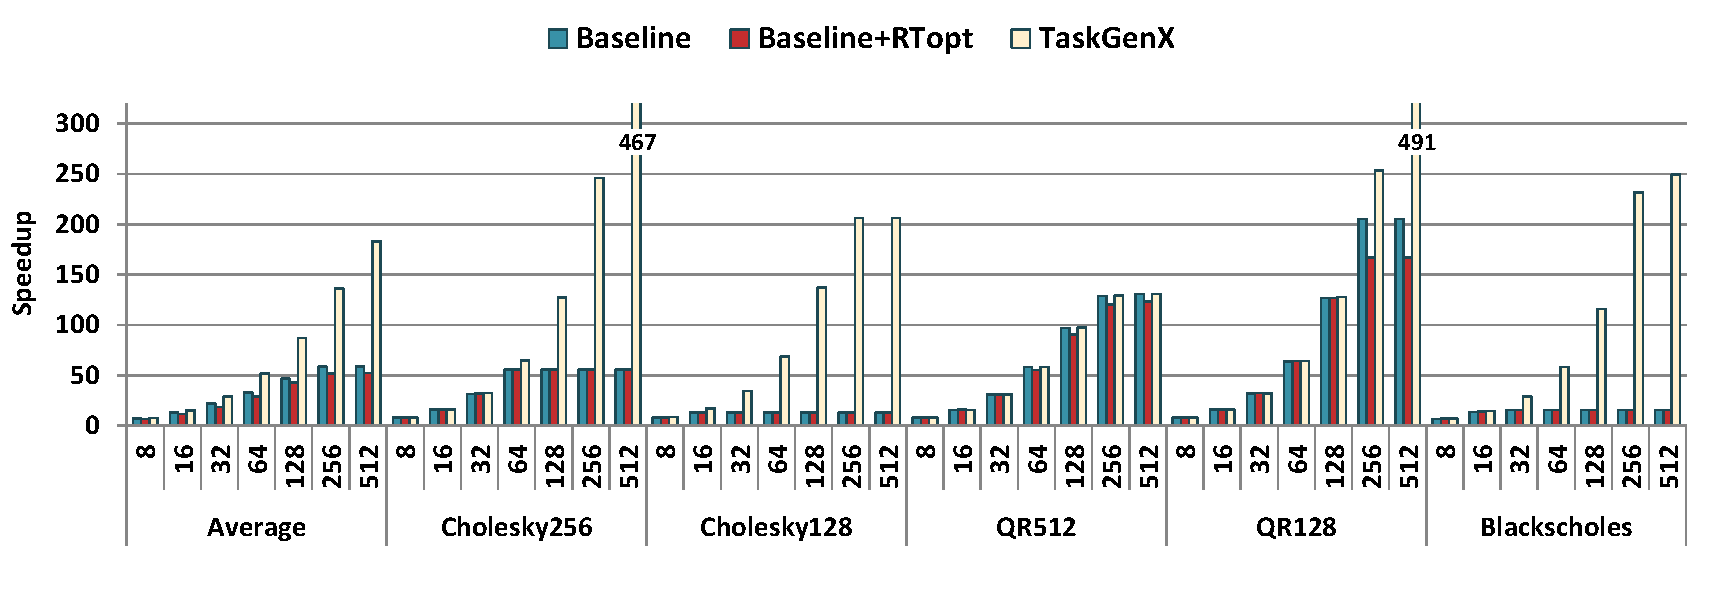
\includegraphics[width=\columnwidth]{figures/speedup_homo.pdf}}
	
	\subfloat[]{\label{fig:speedup_homo2}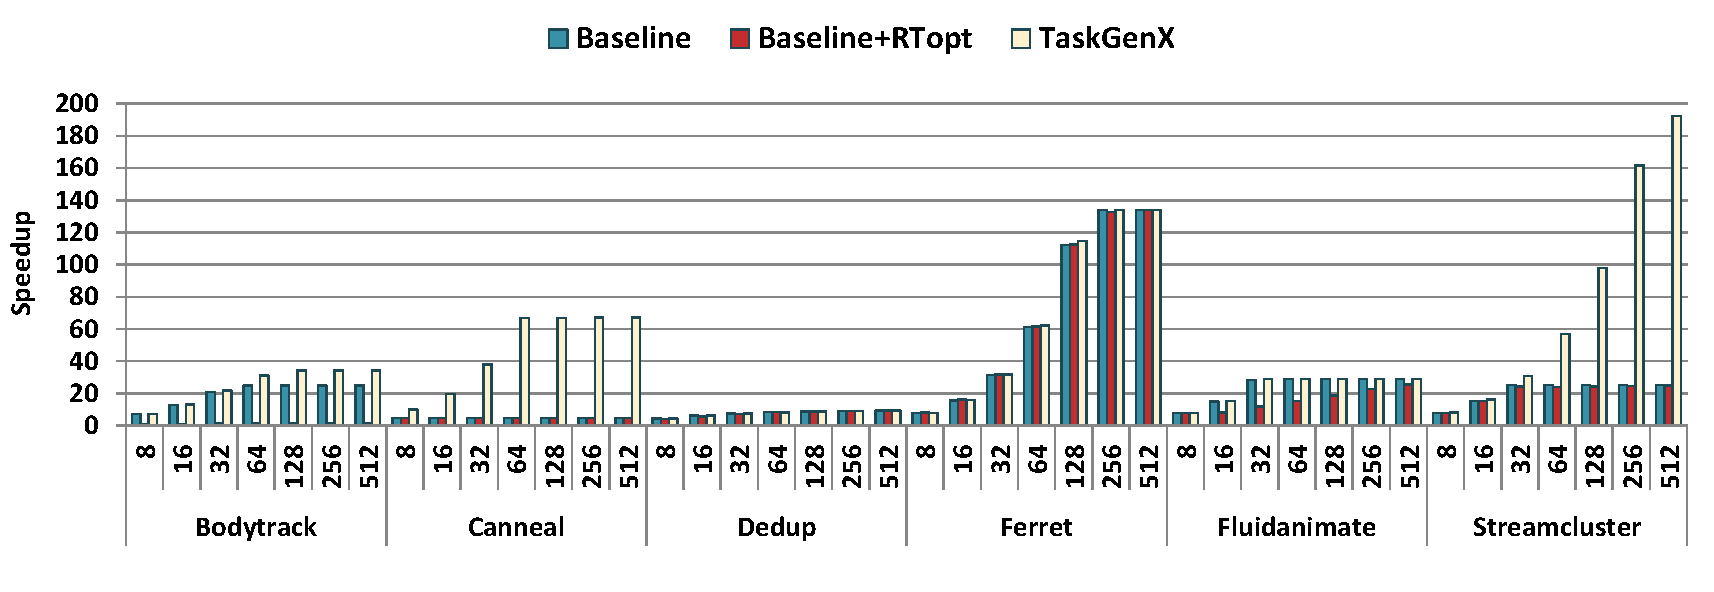
\includegraphics[width=\columnwidth]{figures/speedup_homo2.pdf}}
	\caption{Speedup of {\proposal} compared to the speedup of Baseline and Baseline+RTopt for each application for systems with 8 up to 512 cores. The average results of (a) show the average among all workloads shown on (a) and (b)}
\end{figure}

Figures~\ref{fig:speedup_homo1} and~\ref{fig:speedup_homo2} show the speedup over one core of three different scenarios: 
\begin{itemize}
	\item \textit{Baseline}: the Nanos++ runtime system, which is the default runtime without using any external hardware support
	\item \textit{Baseline+RTopt}: the Nanos++ runtime system that uses the external hardware as if it is a general purpose core 
	\item \textit{{\proposal}}: our proposed runtime system that takes advantage of the optimized hardware
\end{itemize}
We evaluate these approaches with the TaskSim simulator for systems of 8 up to 512 cores.
In the case of Baseline+RTopt the specialized hardware acts as a slow general purpose core that is additional to the number of cores shown on the x axis.
If this core executes a task creation job, it executes it 16$\times$ faster, but as it is specialized for this, we assume that when a task is executed on this core it is executed 4$\times$ slower than in a general purpose core.
The runtime system in this case does not include our modifications that automatically decouple the task creation step for each task.
The comparison against the Baseline+RTopt is used only to show that the baseline runtime is not capable of effectively utilizing the accelerator. 
In most of the cases having this additional hardware without the appropriate runtime support results in slowdown as the tasks are being executed slower on the special hardware.

Focusing on the average results first, we can observe that {\proposal} constantly improves the baseline and the improvement is increasing as the number of cores is increased, reaching up to 3.1$\times$ improved performance on 512 cores. 
This is because as we increase the number of cores, the task creation overhead becomes more critical part of the execution time and affects performance even more.
So, this becomes the main bottleneck due to which the performance of many applications saturates. 
{\proposal} overcomes it by automatically detecting and moving task creation on the specialized hardware.

Looking in more detail, we can see that for all applications the baseline has a saturation point in speedup.
For example Cholesky256 saturates on 64 cores, while QR512 on 256 cores.
In most cases this saturation in performance comes due to the sequential task creation that is taking place for an important percentage of the execution time (as shown in Figure~\ref{fig:master_thread}).
{\proposal} solves this as it efficiently decouples the task creation code and accelerates it leading to higher speedups.

{\proposal} is effective as it either improves performance or it performs as fast as the baseline (there are no slowdowns). 
The applications that do not benefit (QR512, Ferret, Fluidanimate) are the ones with the highest average per task CPU cycles as shown on Table~\ref{tab.apps}.
Dedup also does not benefit as the per task creation cycles are very low compared to its average task size.
Even if these applications consist of many tasks, the task creation overhead is considered negligible compared to the task cost, so accelerating it does not help much. 
%\begin{figure*}[!t]
%\centering

%\begin{figure}[b]
%\begin{tabular}{@{}c@{}}
%  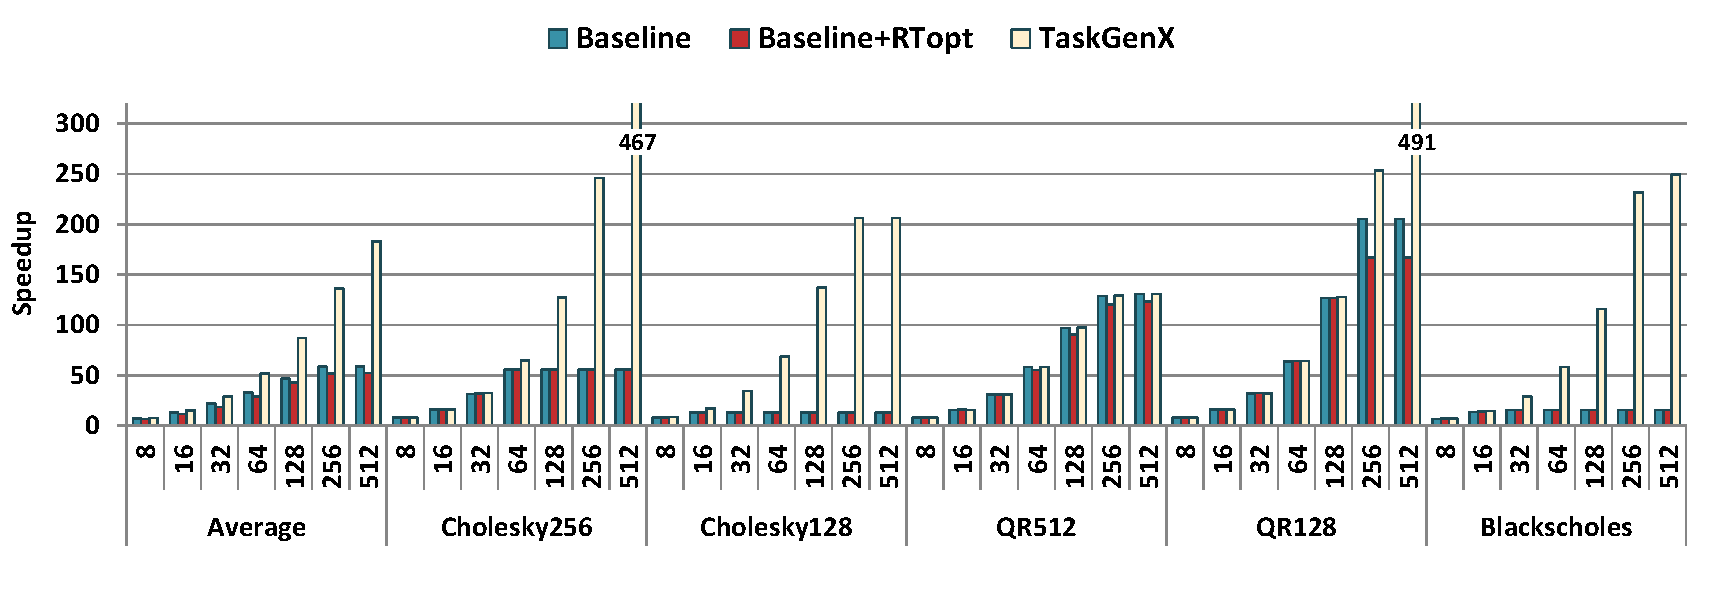
\includegraphics[width=\textwidth]{figures/speedup_homo.pdf}
%  \caption{}
%  \label{fig:speedup_homo1}
%\end{figure}
%
%\begin{figure}[b]
%  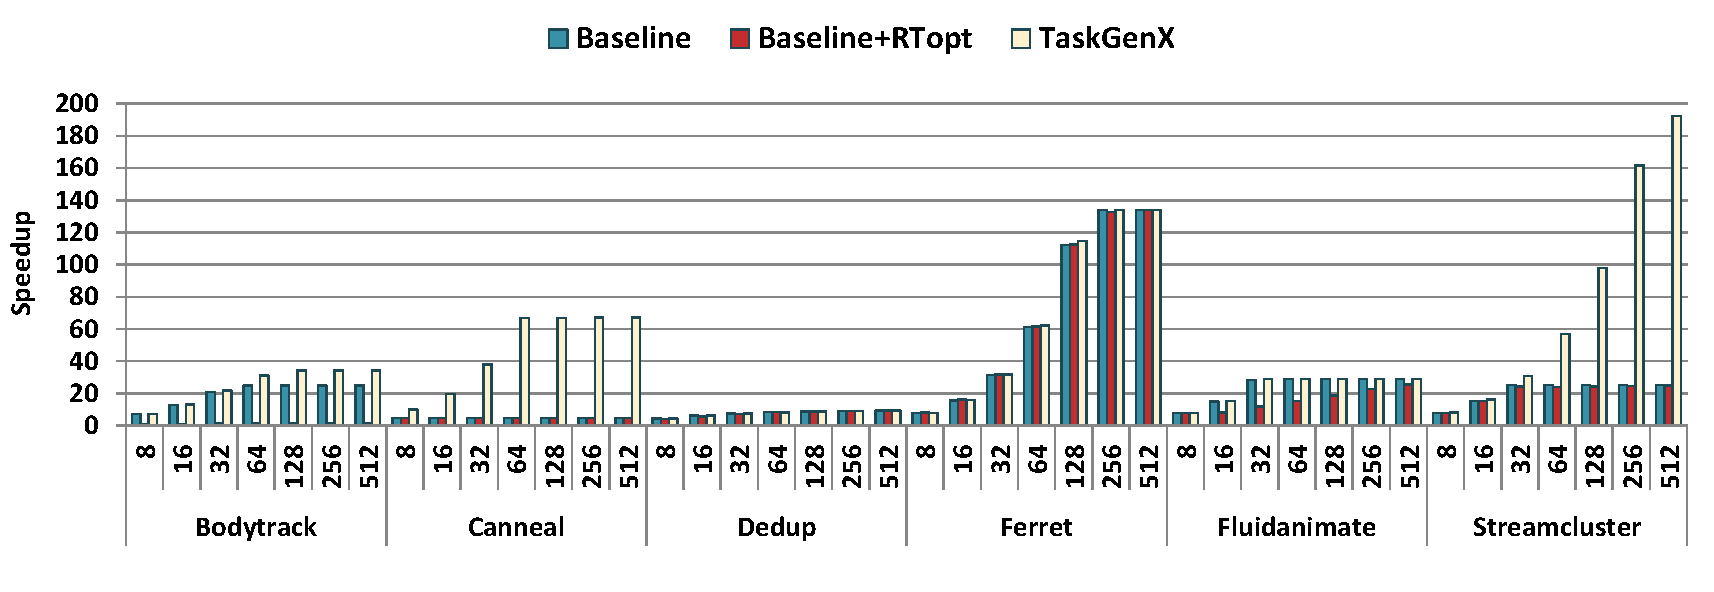
\includegraphics[width=\textwidth]{figures/speedup_homo2.pdf}
%  \caption{}
%  \label{fig:speedup_homo2}
%\end{figure}


This can be verified by the results shown for QR128 workload.
In this case, we use the same input size as QR512 (which is 16K) but we modify the block size, which results in more and smaller tasks.
This not only increases the speedup of the baseline, but also shows even higher speedup when running with {\proposal} reaching very close to the ideal speedup and improving the baseline by 2.3$\times$.
%\begin{figure*}[t]%
%	\centering
%	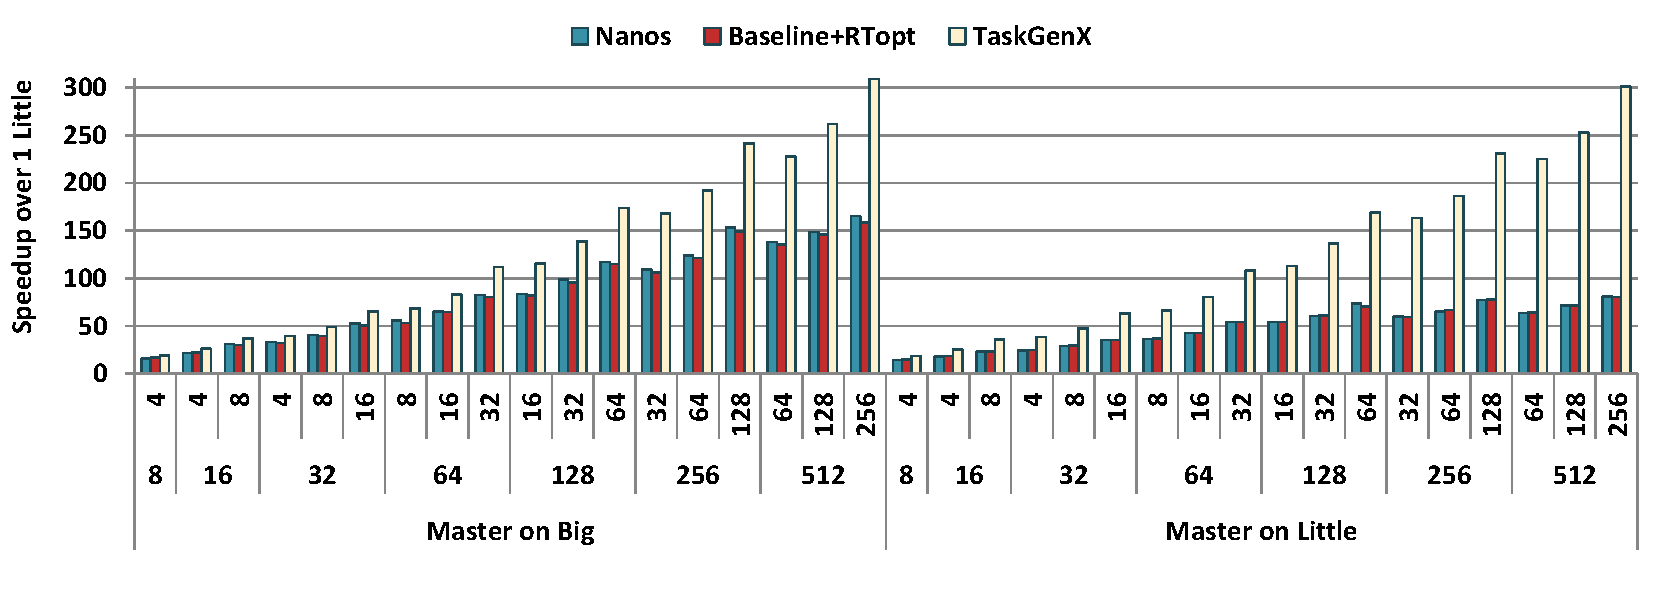
\includegraphics[width=\textwidth]{figures/speedup_hetero_avg.pdf}
%	\caption{Average speedup among all 11 workloads on heterogeneous simulated systems. The numbers at the bottom of x axis show the total number of cores and the numbers above them show the number of big cores. Results are separated depending on the type of core that executes the master thread: a big or little core.}
%	\label{fig:hetero}%
%	\vspace{-0.3cm}
%\end{figure*}
%\begin{figure}[t]%
%	\centering
%	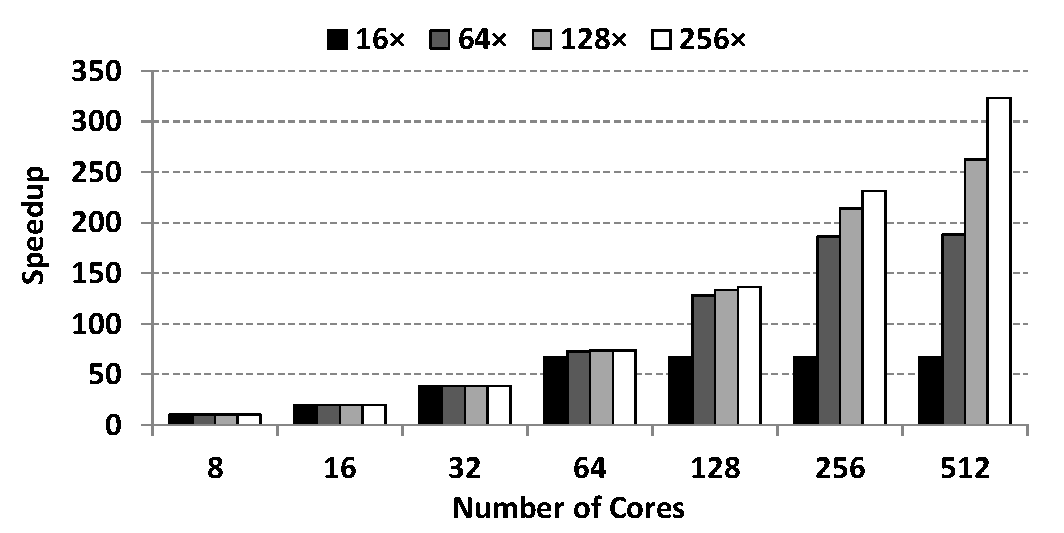
\includegraphics[width=0.6\columnwidth]{figures/canneal_perf.pdf}
%	\caption{Canneal performance as we modify $r$ }
%	\label{fig:canneal}%
%\end{figure}
\begin{figure}[t]
	\centering
	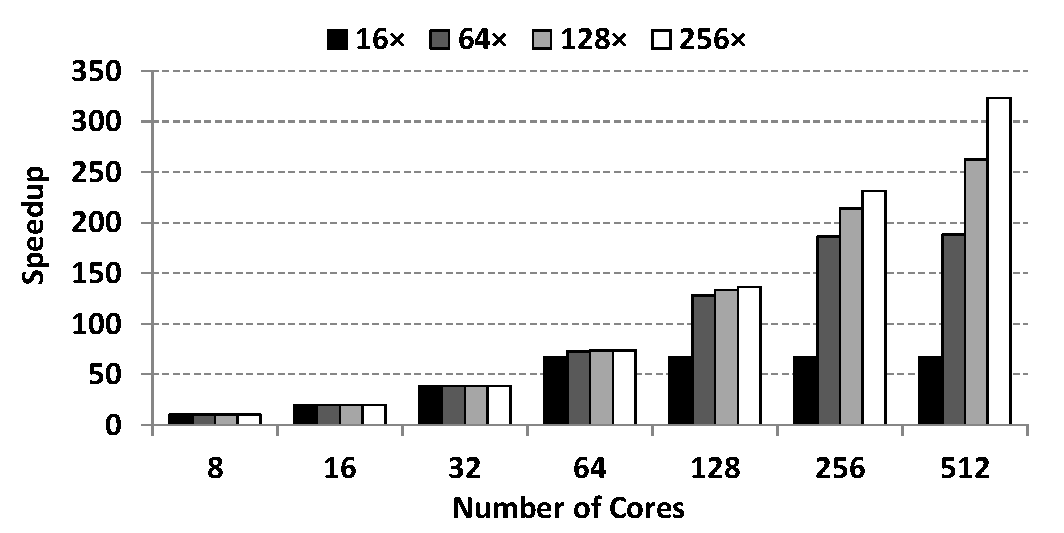
\includegraphics[width=0.75\columnwidth]{figures/canneal_perf.pdf}
	\caption{Canneal performance as we modify $r$; $x$-axis shows the number of cores.}
	\label{fig:canneal}
\end{figure}
Modifying the block size for Cholesky, shows the same effect in terms of {\proposal} over baseline improvement.
However, for this application, using the bigger block size of 256 is more efficient as a whole.
Nevertheless, {\proposal} improves the cases that performance saturates and reaches up to 8.5$\times$ improvement for the 256 block-size, and up to 16$\times$ for the 128 block-size.

Blackscholes and Canneal, are applications with very high task creation overheads compared to the task size as shown on Table~\ref{tab.apps}.
This makes them very sensitive to performance degradation due to task creation. 
As a result their performance saturates even with limited core counts of 8 or 16 cores.
These are the ideal cases for using {\proposal} as such bottlenecks are eliminated and performance is improved by 15.9$\times$ and 13.9$\times$ respectively.
However, for Canneal for which the task creation lasts a bit less than half of the task execution time, accelerating it by 16 times is not enough and soon performance saturates at 64 cores. 
In this case, a more powerful hardware would improve things even more.
Figure~\ref{fig:canneal} shows how the performance of Canneal is affected when modifying the task creation performance ratio, $r$ between the specialized hardware and general purpose.
Using hardware that performs task creation close to 256$\times$ faster than the general purpose core leads to higher improvements.

Streamcluster has also relatively high task creation overhead compared to the average task cost so improvements are increased as the number of cores is increasing.
{\proposal} reaches up to 7.6$\times$ improvement in this case.

The performance of Bodytrack saturates on 64 cores for the baseline. 
However, it does not approach the ideal speedup as its pipelined parallelization technique introduces significant task dependencies that limit parallelism.
{\proposal} still improves the baseline by up to 37\%.
This improvement is low compared to other benchmarks, firstly because of the nature of the application and secondly because Bodytrack introduces nested parallelism.
With nested parallelism task creation is being spread among cores so it is not becoming a sequential overhead as happens in most of the cases.
Thus, in this case task creation is not as critical to achieve better results.
%correct to look at the CREATE overhead value as this is be parallelized among all cores for the 329\,123 tasks of the application. 


\subsection{Heterogeneous Multicore Systems}

%\begin{figure}[t]%
%	\centering
%	\subfloat[Average speedup among all 11 workloads on heterogeneous simulated systems. The numbers at the bottom of x axis show the total number of cores and the numbers above them show the number of big cores. Results are separated depending on the type of core that executes the master thread: a big or little core.]{\label{fig:hetero}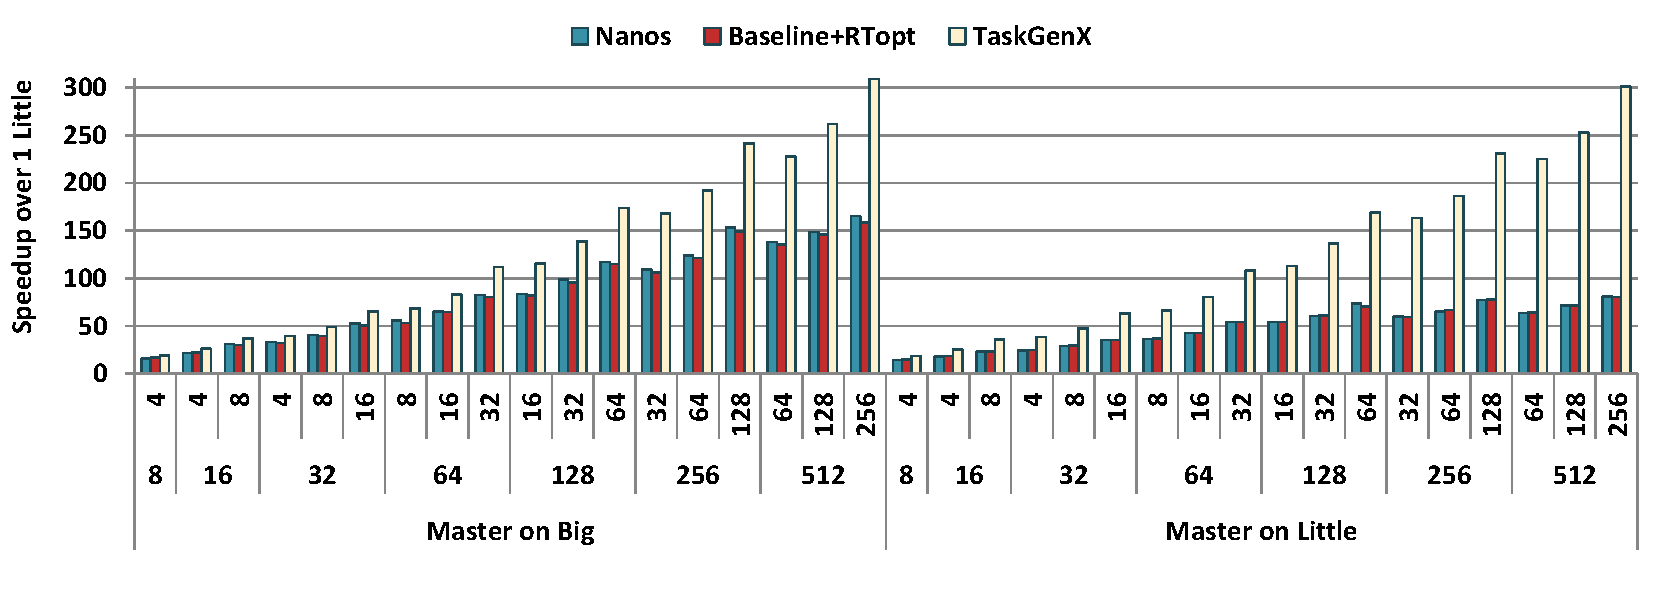
\includegraphics[width=\columnwidth]{figures/speedup_hetero_avg.pdf}}
%	
%	\subfloat[Canneal performance as we modify $r$]{\label{fig:canneal}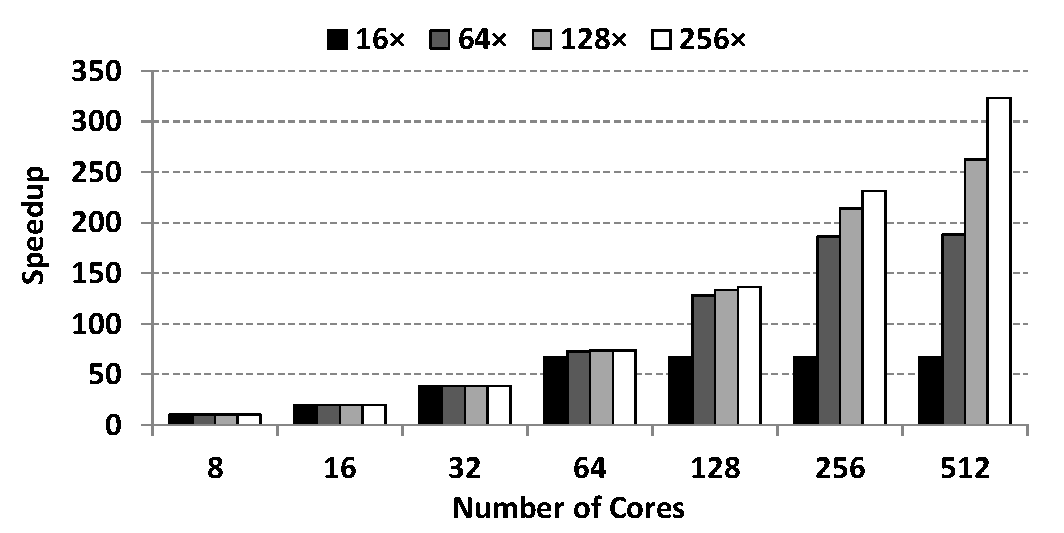
\includegraphics[width=0.5\columnwidth]{figures/canneal_perf.pdf}}
%\subfloat[Average improvement over baseline]{\label{fig:baseline}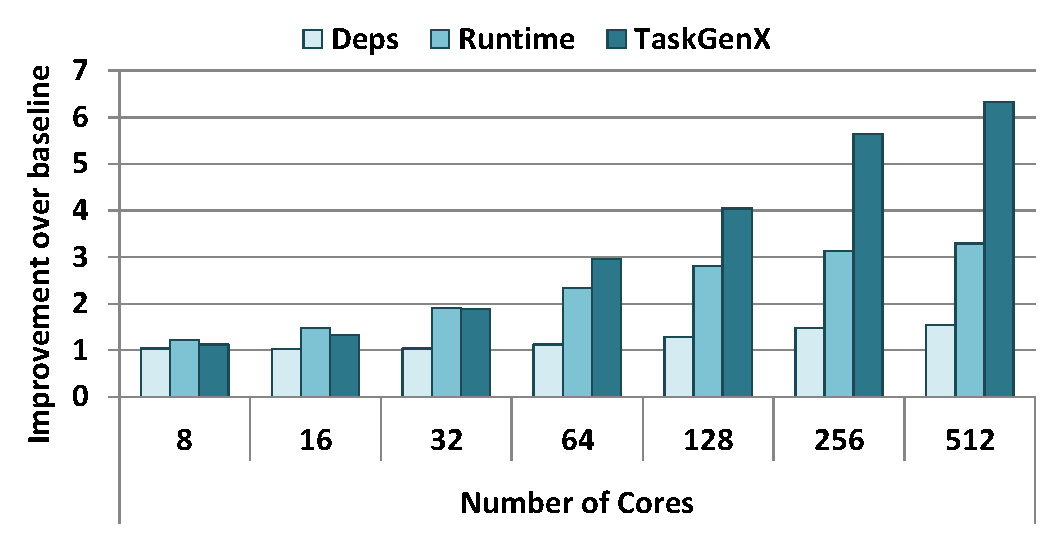
\includegraphics[width=0.48\textwidth]{figures/comparison.pdf}}
%	\vspace{-0.3cm}
%	\caption{X-axis of Figures \ref{fig:canneal} and \ref{fig:baseline} shows the number of cores. For each case an RTopt core is used additionally to the number of cores.}
%\end{figure}

\begin{figure*}[t]%
	\centering
	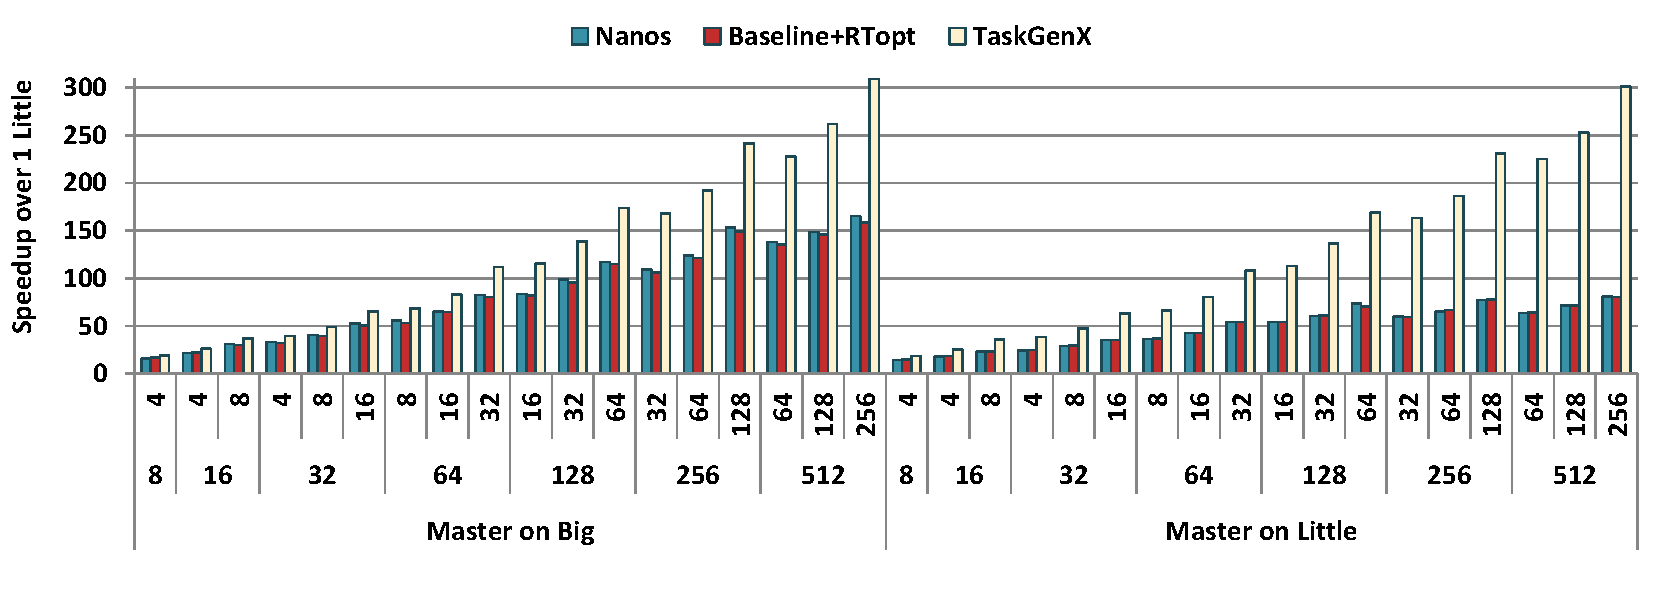
\includegraphics[width=\columnwidth]{figures/speedup_hetero_avg.pdf}
	\caption{Average speedup among all 11 workloads on heterogeneous simulated systems. The numbers at the bottom of x axis show the total number of cores and the numbers above them show the number of big cores. Results are separated depending on the type of core that executes the master thread: a big or little core.}	
	\label{fig:hetero}
\end{figure*}


%	\subfloat[Canneal performance as we modify $r$]{\label{fig:canneal}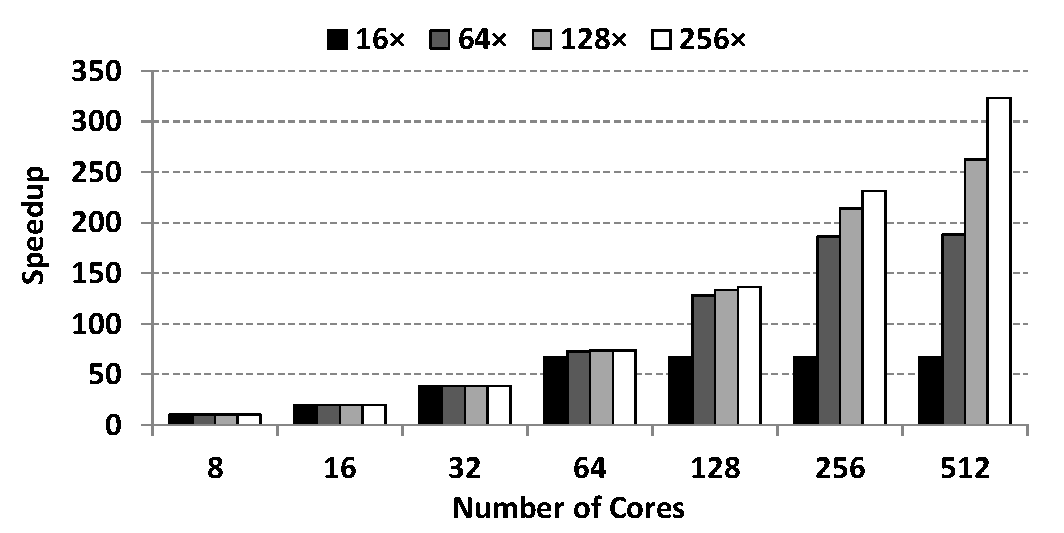
\includegraphics[width=0.5\columnwidth]{figures/canneal_perf.pdf}}
%\subfloat[Average improvement over baseline]{\label{fig:baseline}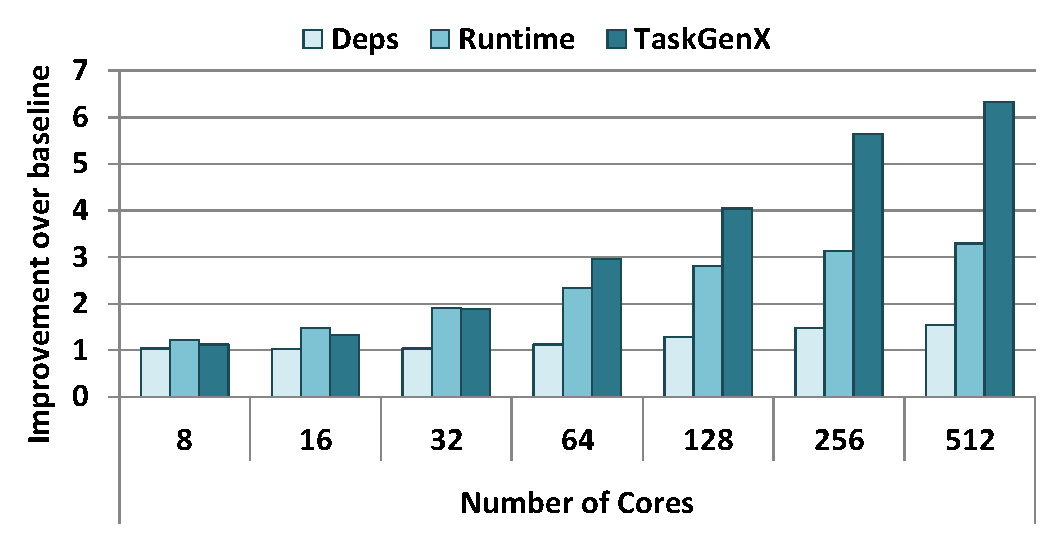
\includegraphics[width=0.48\textwidth]{figures/comparison.pdf}}
%	\vspace{-0.3cm}
%	\caption{X-axis of Figures \ref{fig:canneal} and \ref{fig:baseline} shows the number of cores. For each case an RTopt core is used additionally to the number of cores.}
%\end{figure}


%Figure~\ref{fig:hetero} shows the average speedup obtained among the same applications. 
At this stage of the evaluation our system supports two types of general purpose processors, simulating an asymmetric multi-core processor.
The asymmetric system is influenced by the ARM big.LITTLE architecture~\cite{ARM} that consists of big and little cores.
In our simulations, we consider that the big cores are four times faster than the little cores of the system.
This is based on the average measured performance ratio, shown on Table~\ref{tab.apps}, among the 11 workloads used in this evaluation.
%This assumption is based on prior works~\cite{Chronaki:TPDS} that have shown that for most applications the performance ratio ranges from 3.5$\times$ to 4.5$\times$.

In this set-up there are two different ways of executing a task-based application.
The first way is to start the application's execution on a big core of the system and the second way is to start the execution on a little core of the system.
If we use a big core to load the application, then this implies that the master thread of the runtime system (the thread that performs the task creation when running with the baseline) runs on a fast core, thus tasks are created faster than when using a slow core as a starting point.
We evaluate both approaches and compare the results of the baseline runtime and {\proposal}.

Figure~\ref{fig:hetero} plots the average speedup over one little core obtained among all 11 workloads for the Baseline, Baseline+RTopt and {\proposal}.
The chart shows two categories of results on the x axis, separating the cases of the master thread's execution.
The numbers at the bottom of x axis show the total number of cores and the numbers above show the number of big cores.

%The bars represent the average speedup when running with the baseline runtime or with {\proposal} and the line shows the ideal speedup for each configuration.
%The ideal speedup is the speedup that we would obtain if we were running an application in parallel assuming zero runtime overheads and no dependencies between tasks, technically unachievable for the real applications of our evaluation.
%Equation~\ref{eq.ideal} shows how the ideal speedup is computed for our simulated system where the big cores are four times faster than the little cores.
%\begingroup\makeatletter\def\f@size{9}\check@mathfonts
%\begin{equation}
%  \text{$ideal\_speedup(big, little) = big \times 4 + little$}
%\label{eq.ideal}
%\end{equation}
%\endgroup

The results show that moving the master thread from a big to a little core degrades performance of the baseline.
This is because the task creation becomes even slower so the rest of the cores spend more idle time waiting for the tasks to become ready.
{\proposal} improves performance in both cases.
Specifically when master runs on big, the average improvement of {\proposal} reaches 86\%.
When the master thread runs on a little core, {\proposal} improves performance by up to 3.7$\times$. 
This is mainly due to the slowdown caused by the migration of master thread on a little core.
Using {\proposal} on asymmetric systems achieves approximately similar performance regardless of the type of core that the master thread is running. 
This makes our proposal more portable for asymmetric systems as the programmer does not have to be concerned about the type of core that the master thread migrates.

\subsection{Comparison to Other Approaches}
\begin{figure}[t]
	\centering
	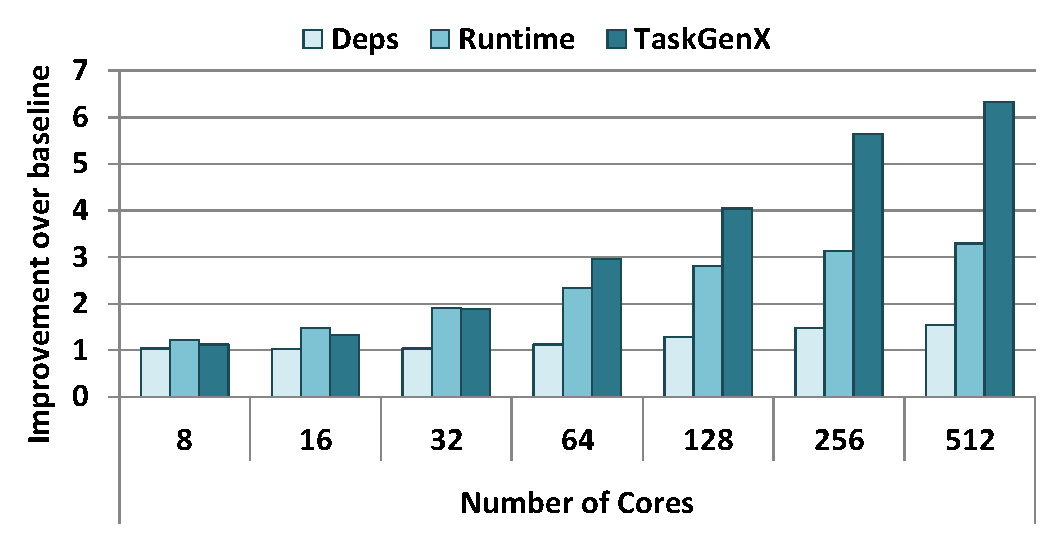
\includegraphics[width=0.75\textwidth]{figures/comparison.pdf}
	\caption{Average improvement over baseline; $x$-axis shows the number of cores.}
	\label{fig:compare}
\end{figure}
%Figure~\ref{fig:comparison} shows the average improvement for each core count over the baseline scheduler. 
As we saw earlier, {\proposal} improves the baseline scheduler by up to 6.3$\times$ for 512 cores.
In this section we compare {\proposal} with other approaches.
To do so, we consider the proposals of Carbon~\cite{Carbon}, Task Superscalar~\cite{TaskSS}, Picos++~\cite{Xubin} and Nexus\#~\cite{Nexus}.
We group these proposals based on the part of the runtime activity they are offloading from the CPU.
Carbon and Task Superscalar are runtime-driven meaning that they both accelerate all the runtime and scheduling parts.
The task creation, dependence analysis as well as the scheduling, namely the ready queue manipulation, are transferred to the RTopt with these approaches. 
These overheads are represented on Table~\ref{tab.apps} under ALL.
For the evaluation of these approaches one RTopt is used optimized to accelerate all the runtime activities. 
The second group of related designs that we compare against is the dependencies-driven, which includes approaches like Picos++ and Nexus\#. 
These approaches aim to accelerate only the dependence analysis part of the runtime as well as the scheduling that occurs when a dependency is satisfied.
The RTopt in this case is optimized to accelerate these activities.
For example, when a task finishes execution, and it has produced input for another task, the dependency tracking mechanism is updating the appropriate counters of the reader task and if the task becomes ready, the task is inserted in the ready queue.
The insertion into the ready queue is the scheduling that occurs with the dependence analysis.
These overheads are represented on Table~\ref{tab.apps} under \textit{Deps+Sched}.

%To compare {\proposal} with other systems, we emulate the behaviour of Carbon~\cite{Carbon} and Picos++~\cite{Xubin} in our system.
%In this emulation, we implement Carbon, that originally accelerates scheduling by using hardware queues. 
%To do so we decouple all the possible scheduling overheads and send them for execution by the accelerator. 
%The average per-task scheduling overheads measured are shown on Table~\ref{tab.apps} under SCHED.
%These overheads might seem high compared to the CREATE overheads that {\proposal} accelerates but they are executed among all threads so at the end they do not induce as much delay as task creation does.
%The difference between our Carbon implementation and the original one is that the original one assumes multiple hardware queues, which enables the parallel manipulation by the threads.
%In our case, we are limited to only one queue, as we want to compare an approach that would be as cheap as the {\proposal} approach and use a single hardware component.

Figure~\ref{fig:compare} shows the average improvement in performance for each core count over the performance of the baseline scheduler on the same core count. 
\textit{Runtime} represents the runtime driven approaches and the \textit{Deps} represents the dependencies driven approaches as described above.
X-axis shows the number of general purpose cores; for every core count one additional RTopt core is used.

Accelerating the scheduling with \textit{Runtime}-driven is as efficient as {\proposal} for a limited number of cores, up to 32.
This is because they both accelerate task creation which is an important bottleneck. 
\textit{Deps}-driven approaches on the other hand are not as efficient since in this case the task creation step takes place on the master thread.

Increasing the number of cores, we observe that the improvement of the \textit{Runtime}-driven over the baseline is reduced and stabilized close to 3.2$\times$ while {\proposal} continues to speedup the execution. 
Transferring all parts of the runtime to RTopt with the  \textit{Runtime}-driven approaches, leads to the serialization of the runtime.
Therefore, all scheduling operations (such as enqueue, dequeue of tasks, dependence analysis etc) that typically occur in parallel during runtime are executed sequentially on the RTopt.
Even if RTopt executes these operations faster than a general purpose core, serializing them potentially creates a bottleneck as we increase the number of cores.
{\proposal} does not transfer other runtime activities than the task creation, so it allows scheduling and dependence analysis operations to be performed in a distributed manner.

%We attribute this to the fact that serializing the scheduling operations becomes a bottleneck when increasing the number of cores.
%Scheduling operations (such as enqueue, dequeue of tasks, dependence analysis etc) generally occur in parallel during runtime, so serializing them for systems of up to 32 cores, is efficient.
%With an increased number of cores it is better to perform scheduling in a distributed manner, just as {\proposal} allows.
%
%Scheduling in general (enqueue, dequeue of tasks, dependence analysis etc) occurs in parallel during runtime.
%TaskGenX does not transfer the scheduling to the special hardware. So scheduling parts are executed on each core whenever they occur on the workers. The other approaches that do move the scheduling on the accelerator they serialize it because we assume that the accelerator is centralized. Is this clear? How could we put it clearly in the text?

%\begin{figure}[t]%
%	\centering
%	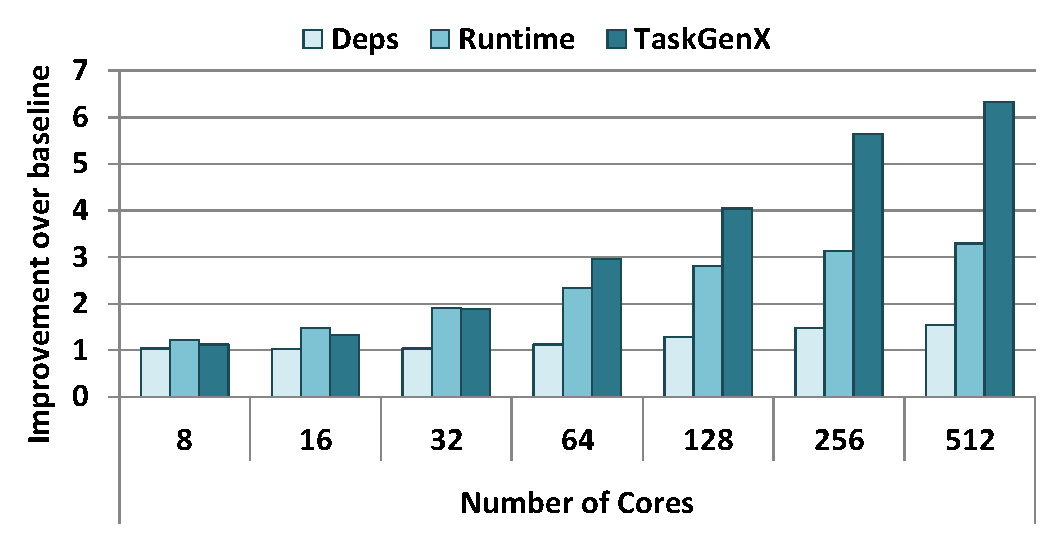
\includegraphics[width=0.6\textwidth]{figures/comparison.pdf}
%	\caption{Average improvement over baseline. X-axis shows the number of cores. For each case an RTopt core is used additionally to the number of cores.}
%	\label{fig:compare}
%	\vspace{-0.3cm}
%\end{figure}

\textit{Deps} driven approaches go through the same issue of the serialization of the dependency tracking and the scheduling that occurs at the dependence analysis stage.
The reason for the limited performance of \textit{Deps} compared to \textit{Runtime} is that \textit{Deps} does not accelerate any part of the task creation. 
Improvement over the baseline is still significant as performance with \textit{Deps} is improved by up to 1.5$\times$.

{\proposal} is the most efficient software-hardware co-design approach when it comes to highly parallel applications.
On average, it improves the baseline by up to 3.1$\times$ for homogeneous systems and up to 3.7$\times$ for heterogeneous systems.
Compared to other state of the art approaches, {\proposal} is more effective on a large number of cores showing higher performance by 54\% over \textit{Runtime} driven approaches and by 70\% over \textit{Deps} driven approaches.


\subsection{Combining TaskGenX with CATS}
\begin{figure*}[t]%
	\centering
	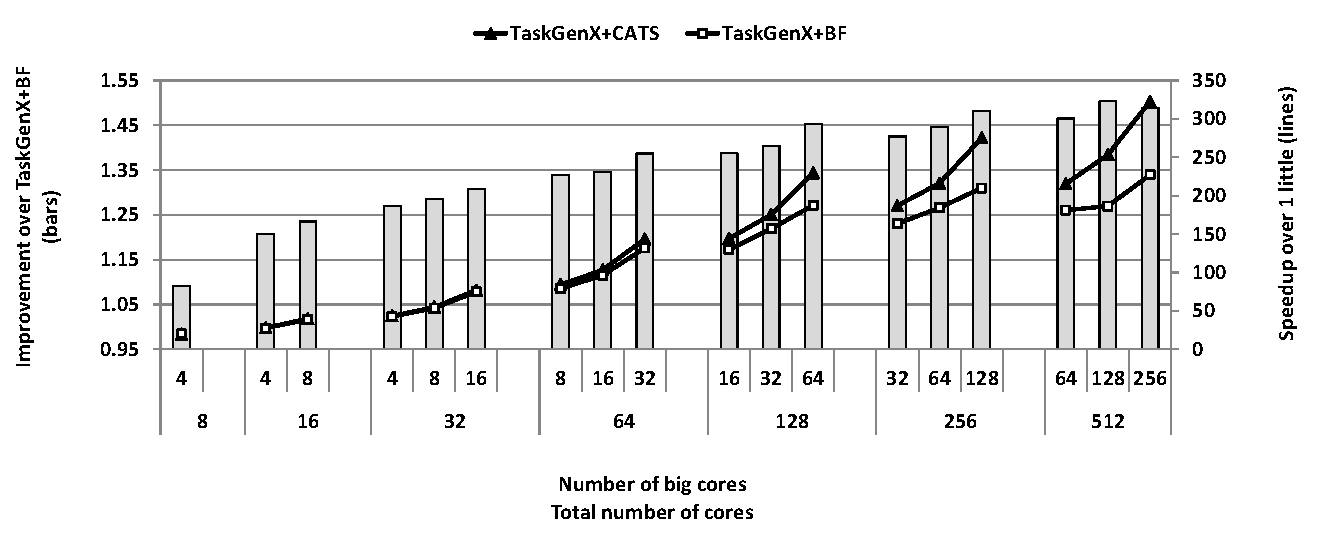
\includegraphics[width=\columnwidth]{figures/TaskGenX+CATS.pdf}
	\caption{Average speedup among 7 dependency synchronized workloads on heterogeneous simulated systems. The numbers at the bottom of x axis show the total number of cores and the numbers above them show the number of big cores.}	
	\label{fig:hetero}
\end{figure*}




%%%%%%%%%%%%%%%%%%%%
%%%%%%%%%%%%%%%%%%%%
%\section{Related Work}
%\label{sec:related}
%%Papers to add:
%1. Flexible Architectural Support for Fine-Grain Scheduling, Kozyrakis
%2. Emilio's papers CATA
%3. Carbon by Kumar et.al.
%4. Xubin's, Jaume's
%5. Nexus
%6. Task superscalar\cite{TaskSS}
Our approach is a new task-based runtime system design that enables the acceleration of task creation to overcome important bottlenecks in performance.
Task-based runtime systems have intensively been studied.
State of the art task-based runtime systems include the OpenMP~\cite{OpenMP}, OmpSs~\cite{OmpSs_PPL11}, StarPU~\cite{starpu} and Swan~\cite{Vandierendonck:PACT2011}.
All these models support tasks and maintain a TDG specifying the inter-task dependencies.
This means that the runtime system is responsible for the task creation, the dependence analysis as well as the scheduling of the tasks.
However, none of these runtime systems offers automatic offloading of task creation.

The fact that task-based programming models are so widely spread makes approaches like ours very important and also gives importance to studies that focus on adding hardware support to boost performance of task-based runtime systems.
%on how to boost performance of such programming models with hardware support.
%Many works in the research community focus on adding hardware support to boost performance of task-based runtime systems by reducing the runtime overheads.
Even if their work focuses more on the hardware part of the design, their contributions are very relative to our study as we can distinguish which parts of the hardware is more beneficial to be accelerated.

Carbon~\cite{Carbon} accelerates the scheduling of tasks by implementing hardware ready queues.
Carbon maintains one hardware queue per core and accelerates all possible scheduling overheads by using these queues.
Nexus\#~\cite{Nexus} is also a distributed hardware accelerator capable of executing the \textit{in}, \textit{out}, \textit{inout}, \textit{taskwait} and \textit{taskwait on} pragmas, namely the task dependencies.
Unlike Carbon and Nexus, {\proposal} accelerates only task creation.
Moreover, ADM~\cite{Sanchez:2010} is another distributed approach that proposes hardware support for the inter-thread communication to avoid going through the memory hierarchy. 
This aims to provide a more flexible design as the scheduling policy can be freely implemented in software.
These designs require the implementation of a hardware component for each core of an SoC.
Our proposal assumes a centralized hardware unit that is capable of operating without the need to change the SoC.

Task Superscalar~\cite{TaskSS} and Picos++~\cite{Xubin} use a single hardware component to accelerate parts of the runtime system.
In the case of Task superscalar, all the parts of the runtime system are transferred to the accelerator.
Picos++~\cite{Xubin} is a hardware-software co-design that supports nested tasks. 
This design enables the acceleration of the inter-task dependencies on a special hardware.
Swarm~\cite{Swarm} performs speculative task execution. 
Instead of accelerating parts of the runtime system, Swarm uses hardware support to accelerate speculation.
This is different than our design that decouples only task creation.

%In our paper we present a flexible runtime system that supports the acceleration of task creation.
Our work diverges to prior studies for two main reasons:
\begin{itemize}
\item The implementation of prior studies requires changes in hardware of the SoC.
This means that they need an expensive design where each core of the chip has an extra component.
Our proposal offers a much cheaper solution by requiring only a single specialized core that, according to our experiments, can manage the task creation for 512-core SoCs.
\item None of the previous studies is aiming at accelerating exclusively task creation overheads. 
According to our study task creation becomes the main bottleneck as we increase the number of cores and our study is the first that takes this into account.
\end{itemize}




%%%%%%%%%%%%%%%%%%%
%%%%%%%%%%%%%%%%%%%
\section{Conclusions}
\label{sec.taskgenx.conclusions}
This paper presented {\proposal}, the first software-hardware co-design that decouples task creation and accelerates it on a runtime optimized hardware.
In contrast to previous studies, our paper makes the observation that task creation is a significant bottleneck in parallel runtimes.
Based on this we implemented {\proposal} on top of the OpenMP programming model.
%Task creation overheads are notable especially in workloads with fine grained parallelism.
%The more we increase the granularity and the number of cores, the more critical the task creation becomes.
On the hardware side, our paper sets the requirements for the RTopt in order to achieve optimal results and proposes an asymmetric architecture that combines it with general purpose cores.

Based on this analysis we evaluate the performance of 11 real workloads using our approach with TaskSim simulator.
Accelerating task creation, {\proposal} achieves up to 15.8$\times$ improvement (Cholesky128) over the baseline for homogeneous systems and up to 16$\times$ (Blackscholes) on asymmetric systems when the application is launched on a little core.
%We showed that applications with fine grained parallelism are more prone to exhibit task creation overheads and {\proposal} manages to 
%achieve higher improvements in these cases where task creation is more important.
%7$\times$ on asymmetric systems when the application is launched on a little core.
% 6$\times$ average improvement
Using {\proposal} on asymmetric systems offers a portable solution, as the task creation is not affected by the type of core that the master thread is bound to.


We further showed that for some cases like Canneal where task creation needs to be accelerated as much as 197$\times$ in order to steadily provide enough created tasks for execution.
However, even by using a realistic and implementable hardware approach that offers 16$\times$ speedup of task creation, achieves satisfactory results as it improves the baseline up to 14$\times$.

Comparing {\proposal} against other approaches such as Carbon, Nexus, Picos++ or TaskSuperscalar that manage to transfer different parts of the runtime to the RTopt proves that {\proposal} is the most minimalistic and effective approach.
Even if {\proposal} transfers the least possible runtime activity to the RTopt hardware it achieves better results.
This implies that {\proposal} requires a less complicated hardware accelerator, as it is specialized for only a small part of the runtime, unlike the other approaches that need specialization for task creation, dependency tracking and scheduling.

%FUTURE work...
We expect that combining {\proposal} with an asymmetry-aware task scheduler will achieve even better results, as asymmetry introduces load imbalance.


%From our study we obtain interesting conclusions such as:
%\begin{itemize}
%\item The bigger the tasks the less important the task creation overheads
%\item {\proposal} makes current programming models more portable when running on asymmetric systems as the programmer does not have to worry for the type of core that launches the application
%\item Accelerating task creation is actually the most critical point to achieve high performance in many core systems as from other approaches we saw that they do not scale so well compared to {\proposal}
%\item Current task-based programming models suffer from task creation
%\end{itemize}

